\documentclass[11pt,a4paper]{article}
\usepackage[utf8]{inputenc}
\usepackage[T1]{fontenc}
\usepackage[spanish,es-noshorthands,es-tabla]{babel}
\usepackage{lmodern}
\usepackage{amsmath,amssymb,amsthm}
\usepackage{graphicx}
\usepackage{booktabs}
\usepackage{geometry}
\usepackage{caption}
\usepackage{subcaption}
\usepackage{float}
\usepackage{xcolor}
\usepackage[colorlinks=true,linkcolor=blue!50!black,citecolor=blue!50!black,urlcolor=blue!50!black]{hyperref}
\geometry{margin=2.5cm}
\graphicspath{{../figures/}}
\captionsetup{font=small,labelfont=bf}
\emergencystretch=3em

\newcommand{\R}{\mathbb{R}}
\newcommand{\code}[1]{\texttt{#1}}

\title{Aproximaciones numéricas de problemas con \emph{blow-up}:\\
reimplementación en Python de los experimentos y nuevos resultados}
\author{Julián Fernández Bonder}
\date{\today}

\begin{document}
\maketitle

\begin{abstract}
Este informe describe la reimplementación en Python (NumPy/SciPy) de los
experimentos numéricos de siete artículos sobre aproximaciones numéricas de
problemas con explosión en tiempo finito: ecuaciones parabólicas con
condiciones de borde no lineales, ecuaciones diferenciales estocásticas y una
ecuación en derivadas parciales estocástica. Los códigos originales, escritos
en MATLAB, se habían perdido. En los artículos con experimentos se
reprodujeron sus figuras y tablas; en los trabajos teóricos se diseñaron
experimentos que ilustran los teoremas. Se agregan además algunos
experimentos nuevos (el umbral de explosión para $u_t=u_{xx}+u^p$ con
condiciones de Dirichlet, un corte de la variedad estable, la ley
exponencial del tiempo de explosión en la SPDE) y un paquete de paso
temporal adaptativo para problemas con explosión. Todo el código, las
figuras y este informe están en el repositorio \code{jfbonder/blow-up}.
\end{abstract}

\tableofcontents

%======================================================================
\section{Introducción}

\subsection{Objetivo y organización}

Los artículos considerados son \cite{AFR,FR,FGR,AFGR-dims,AFGR-sys,DFGRS,FG}.
Los resultados se agrupan por tema:
\begin{itemize}
\item \textbf{Problemas parabólicos} (Sección~\ref{sec:parab}): la ecuación
del calor con flujo no lineal en el borde y su semidiscretización
\cite{AFR,FR,FGR,AFGR-dims,AFGR-sys}.
\item \textbf{Ecuaciones estocásticas} (Sección~\ref{sec:estoc}): EDEs con
explosión \cite{DFGRS} y la ecuación de reacción-difusión con ruido blanco
espacio-temporal \cite{FG}.
\item \textbf{Paso temporal adaptativo} (Sección~\ref{sec:adapt}): un paquete
general con la regla de paso de los artículos.
\end{itemize}
La Sección~\ref{sec:discrepancias} reúne las discrepancias con los
artículos y las erratas encontradas, y la Sección~\ref{sec:repro} explica
cómo reproducir cada resultado.

De los siete artículos, sólo tres contienen experimentos numéricos
(\cite{AFR,DFGRS,FG}); los otros cuatro son teóricos. Para cada artículo
hay en el repositorio una nota (\code{papers/notes/}) con el problema, el
esquema numérico, los teoremas y todo lo que el artículo no especifica.

\subsection{El código}

El paquete \code{blowup} tiene cuatro módulos:
\begin{itemize}
\item \code{blowup.parabolic}: semidiscretizaciones P1 con
\emph{mass lumping} en una dimensión (flujo no lineal en el borde, Dirichlet
con reacción, sistemas acoplados), sistemas generales $MU'=-AU+BU^p$ con
diferencias finitas en el cuadrado, clasificación decaimiento/explosión,
bisección para umbrales e integración hasta muy cerca del tiempo de
explosión.
\item \code{blowup.sode}: Euler--Maruyama adaptativo para EDEs.
\item \code{blowup.spde}: diferencias finitas con ruido blanco
espacio-temporal y paso adaptativo.
\item \code{blowup.adaptive}: el paquete de paso adaptativo
(Sección~\ref{sec:adapt}).
\end{itemize}
Los experimentos están en \code{experiments/}, un script por figura o grupo
de figuras, y hay 24 tests automáticos en \code{tests/}.

\subsection{Integración hasta el tiempo de explosión}\label{sec:rescaling}

Varios experimentos requieren distinguir nodos que explotan de nodos que
quedan acotados, o medir tasas de explosión. Para eso hay que acercarse
mucho a $T_h$: un nodo que explota como $-\ln(T_h-t)$ sólo se distingue de
uno acotado si $T_h-t$ recorre muchas décadas. Se usa el cambio de variable
\[
\frac{dt}{ds}=g(U)=\frac{1}{\max\big(1,\psi(U)\big)},\qquad
\frac{dU}{ds}=g(U)\,F(U),
\]
que es la versión continua de la regla de paso adaptativo de los artículos
(para $F$ con no linealidad $u^p$, $\psi(U)=\|U\|_\infty^{p-1}$). En la
variable $s$ la solución crece exponencialmente y $t(s)\to T_h$. La clave
numérica es calcular el tiempo restante como
\[
T_h-t(s)=\int_s^\infty g(U(\sigma))\,d\sigma,
\]
integrando hacia atrás desde el final (cada tramo se integra en forma exacta
para una exponencial, más una cola geométrica), en lugar de restar
$T_h-t$, que pierde toda la precisión cuando $T_h-t\ll10^{-16}$. Así se
llega a $T_h-t\approx10^{-60}$--$10^{-270}$ con precisión relativa
completa. Las ecuaciones en $s$ se integran con LSODA o BDF con
\code{rtol}$=10^{-9}$--$10^{-10}$.

En lo que sigue, un nodo \emph{explota} si sigue creciendo en las últimas
diez décadas de $T_h-t$; un nodo acotado no cambia en ese intervalo (a
precisión de máquina).

%======================================================================
\section{Problemas parabólicos}\label{sec:parab}

\subsection{El esquema común}

Salvo indicación en contrario, se considera
\[
u_t=u_{xx}+r(u)\ \text{en }(0,1),\qquad u_x(0,t)=0,\qquad u_x(1,t)=F(u(1,t)),
\]
semidiscretizada con elementos finitos P1 y \emph{mass lumping} en la malla
uniforme $x_i=i/N$, $h=1/N$:
\begin{align*}
u_0'&=\tfrac{2}{h^2}(u_1-u_0)+r(u_0),\\
u_i'&=\tfrac{1}{h^2}(u_{i+1}-2u_i+u_{i-1})+r(u_i),\qquad 1\le i\le N-1,\\
u_N'&=\tfrac{2}{h^2}(u_{N-1}-u_N)+\tfrac{2}{h}F(u_N)+r(u_N).
\end{align*}
Para los sistemas rígidos se usan integradores implícitos con jacobiano
exacto.

%----------------------------------------------------------------------
\subsection{Variedad estable \cite{AFR}}

\paragraph{Problema.} $u_t=u_{xx}$, $u_x(0)=0$, $u_x(1)=u^p-u$, con dato
$\lambda u_0$. Los únicos estados estacionarios son $u\equiv0$ y $u\equiv1$.
Existe $\lambda_{c,h}$ tal que la solución decae a cero si
$\lambda<\lambda_{c,h}$, explota si $\lambda>\lambda_{c,h}$ y converge a
$1$ si $\lambda=\lambda_{c,h}$. Experimentos del artículo: $p=2$,
$u_0=\frac12\cos(2\pi x)+1$.

\paragraph{Método.} $\lambda_{c,h}$ se calcula por bisección hasta
$10^{-9}$. Cada $\lambda$ se clasifica con criterios rigurosos por el
principio de comparación (Teorema~3.1 de \cite{AFR}): decaimiento si
$\max u<0.99$ y explosión si $\min u>1.01$. Integración con LSODA, jacobiano
exacto y \code{rtol}$=10^{-10}$.

\paragraph{Resultados.} La Tabla~\ref{tab:afr} compara con la Tabla~1 del
artículo. Para $N=50$ y $N=100$ los valores coinciden; para $N=10$ y $N=20$
hay una diferencia de $\sim10^{-3}$ que no se pudo explicar (se probaron
tolerancias tipo \code{ode45}, bordes de primer orden, matriz de masa
consistente y otras discretizaciones del dato). El orden de convergencia
observado es exactamente $2$ (Figura~\ref{fig:afr}), lo que confirma la
conjetura del artículo, y por extrapolación de Richardson
$\lambda_c\approx0.9770294$. El autovalor inestable de la linealización en
$(1,\dots,1)$ converge al continuo $k^2$ con $k\tanh k=p-1$ ($1.43920$ para
$N=100$ contra $1.43923$).

\begin{table}[H]
\centering
\begin{tabular}{rccc}
\toprule
$N$ & $\lambda_{c,h}$ (Python) & Tabla 1 de \cite{AFR} & autovalor inestable $\mu_h$\\
\midrule
10 & 0.976472 & 0.9755 & 1.43617\\
20 & 0.976894 & 0.9766 & 1.43846\\
50 & 0.977008 & 0.9770 & 1.43911\\
100 & 0.977024 & 0.9770 & 1.43920\\
200 & 0.977028 & -- & 1.43922\\
400 & 0.977029 & -- & 1.43923\\
\midrule
límite & 0.9770294 & & 1.43923\\
\bottomrule
\end{tabular}
\caption{Valor crítico $\lambda_{c,h}$ para $p=2$, $u_0=\frac12\cos(2\pi x)+1$.}
\label{tab:afr}
\end{table}

\begin{figure}[H]
\centering
\begin{subfigure}{0.48\textwidth}
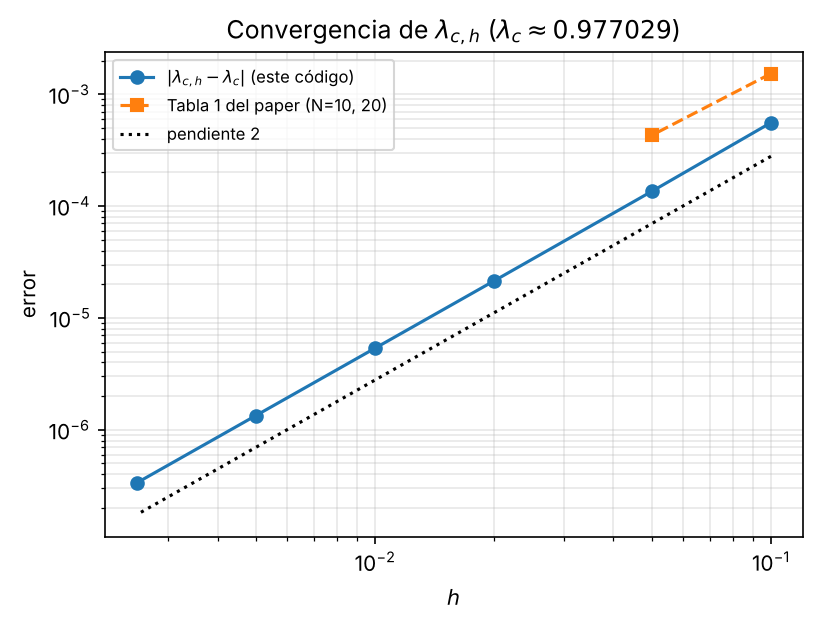
\includegraphics[width=\textwidth]{parabolic/stable_manifold_lambda_convergence.png}
\caption{Convergencia de $\lambda_{c,h}$: orden 2.}
\end{subfigure}\hfill
\begin{subfigure}{0.48\textwidth}
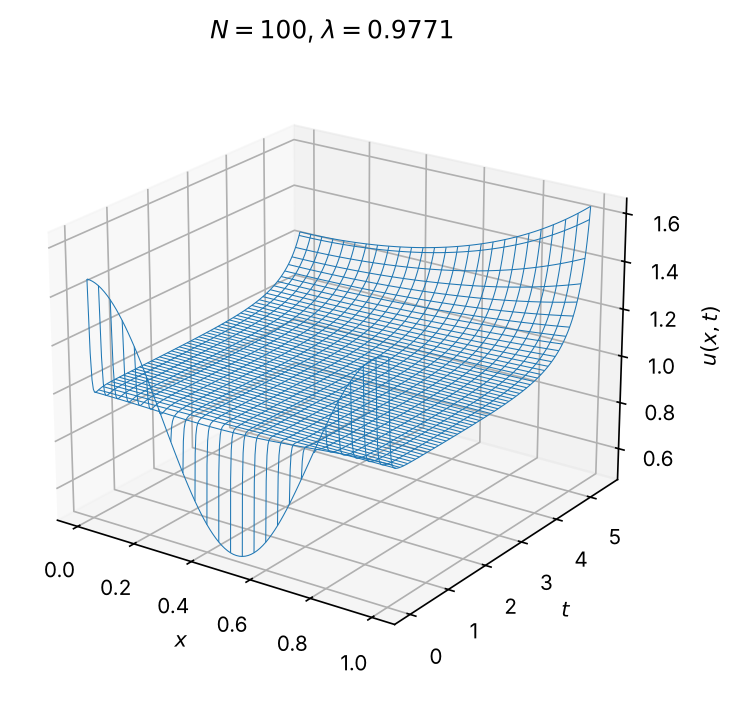
\includegraphics[width=\textwidth]{parabolic/stable_manifold_fig1.png}
\caption{Figura 1 de \cite{AFR}: $N=100$, $\lambda=0.9771$.}
\end{subfigure}
\caption{Variedad estable. A la derecha, la solución se aplana cerca de
$u\equiv1$, permanece allí hasta $t\approx4.5$ y luego despega, primero en
$x=1$.}
\label{fig:afr}
\end{figure}

\paragraph{Experimento nuevo: un corte de la variedad estable.} En el plano
de datos $u_0=a+b\cos(2\pi x)$ se calcula, para cada $b$, el valor crítico
$a^*(b)$; la curva es la intersección de la variedad estable discreta con
ese plano (Figura~\ref{fig:slice}). Ya con $N=10$ la curva está casi
superpuesta con la de $N=100$, y el rayo de la Tabla~1 la corta en
$(\lambda_c/2,\lambda_c)$.

\begin{figure}[H]
\centering
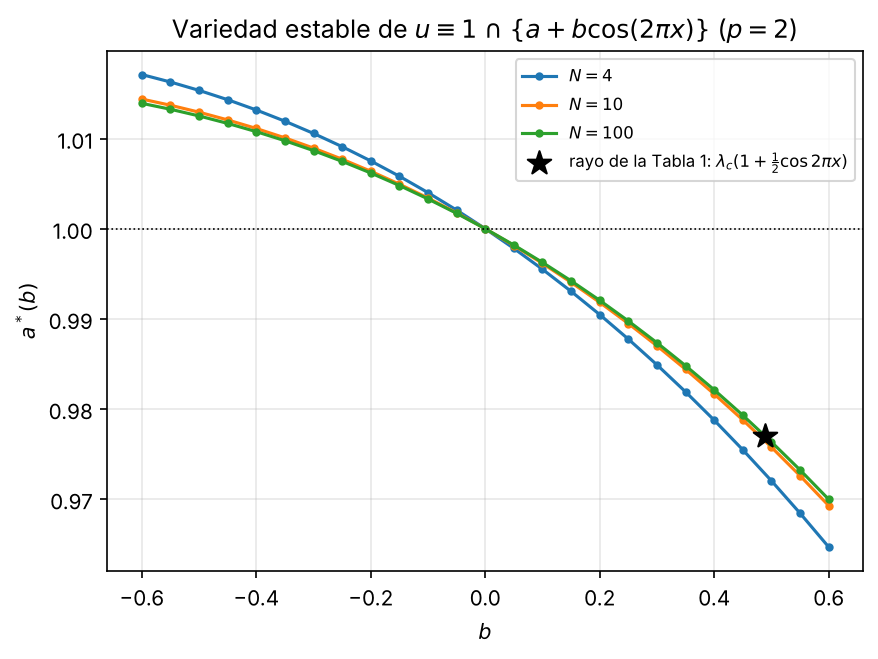
\includegraphics[width=0.6\textwidth]{parabolic/stable_manifold_slice.png}
\caption{Variedad estable de $u\equiv1$ intersecada con el plano
$\{a+b\cos(2\pi x)\}$.}
\label{fig:slice}
\end{figure}

\paragraph{Experimento nuevo: $u_t=u_{xx}+u^p$ con Dirichlet.} El mismo
fenómeno aparece para $u_t=u_{xx}+u^p$ en $(0,1)$ con $u(0)=u(1)=0$, donde
hay una única estacionaria positiva $v$. Para $p=2$,
\[
\max v=\Big(2\sqrt{\tfrac{p+1}{2}}\,J\Big)^{2/(p-1)}\approx11.7967,\qquad
J=\tfrac{1}{p+1}B\big(\tfrac{1}{p+1},\tfrac12\big).
\]
La estacionaria discreta $V_h$ se calcula por Newton y $\lambda_{c,h}$ por
bisección, comparando nodo a nodo con $V_h$ (decaimiento si $U<0.99\,V_h$,
explosión si $U>1.01\,V_h$). La convergencia es de orden $h^2$ para los dos
datos estudiados (Tabla~\ref{tab:dir}); la linealización en $V_h$ tiene un
único autovalor positivo, $\mu\approx9.976$, de modo que la variedad estable
tiene codimensión uno. Con $\lambda=\lambda_{c,h}(1\pm10^{-k})$ la solución
pasa un tiempo $\approx k\ln10/\mu$ cerca de $v$ antes de decaer o explotar
(Figura~\ref{fig:dir}).

\begin{table}[H]
\centering
\begin{tabular}{rcccc}
\toprule
$N$ & $\max V_h$ & $\mu_h$ & $\lambda_{c,h}$ ($\sin\pi x$) & $\lambda_{c,h}$ ($\frac{27}{4}x(1-x)^2$)\\
\midrule
10 & 11.7117 & 9.9029 & 11.410893 & 12.890662\\
50 & 11.7933 & 9.9733 & 11.510482 & 13.007673\\
100 & 11.7958 & 9.9755 & 11.513566 & 13.011310\\
400 & 11.7966 & 9.9762 & 11.514530 & 13.012446\\
\midrule
límite & 11.7967 & & 11.514594 & 13.012522\\
\bottomrule
\end{tabular}
\caption{Umbral para $u_t=u_{xx}+u^2$ con Dirichlet.}
\label{tab:dir}
\end{table}

\begin{figure}[H]
\centering
\begin{subfigure}{0.55\textwidth}
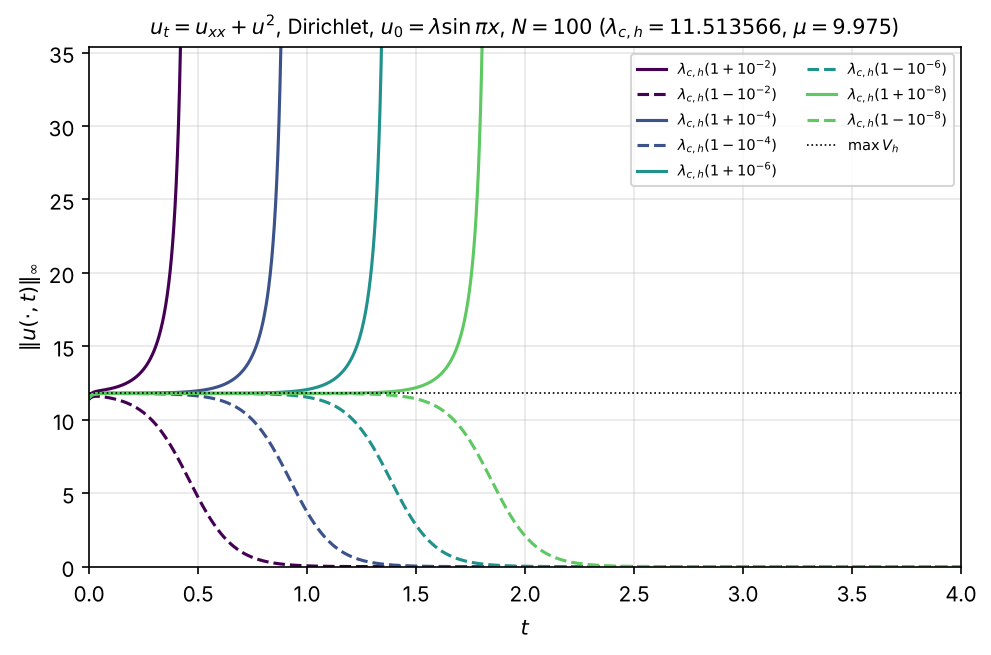
\includegraphics[width=\textwidth]{parabolic/dirichlet_threshold_dynamics.png}
\end{subfigure}\hfill
\begin{subfigure}{0.43\textwidth}
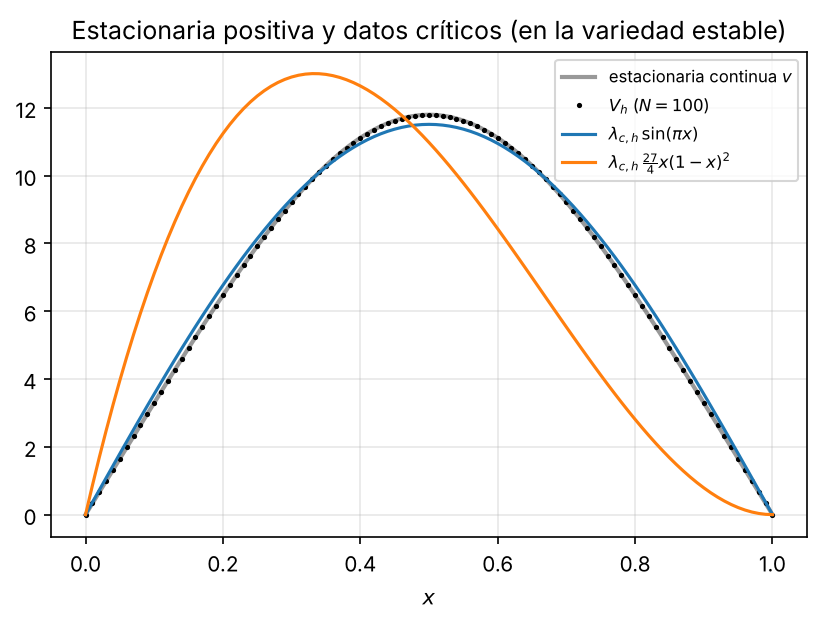
\includegraphics[width=\textwidth]{parabolic/dirichlet_threshold_profiles.png}
\end{subfigure}
\caption{Izquierda: $\|u(\cdot,t)\|_\infty$ para $\lambda$ cerca de
$\lambda_{c,h}$; cada factor $100$ de cercanía al umbral agrega
$\approx0.46$ unidades de tiempo cerca de $v$. Derecha: estacionaria y datos
críticos.}
\label{fig:dir}
\end{figure}

%----------------------------------------------------------------------
\subsection{Conjuntos de blow-up numéricos \cite{FGR}}

\paragraph{Problema.} $u_t=u_{xx}$, $u_x(0)=0$, $u_x(1)=f(u(1))$. El
Teorema~1 de \cite{FGR} afirma que la cantidad de nodos que explotan depende
sólo de $f$ y no de $h$. El artículo es teórico.

\paragraph{Resultados.} Para $f=s^p$ se integra hasta $T_h-t\sim10^{-60}$--$10^{-200}$
(Sección~\ref{sec:rescaling}). La cantidad de nodos que explotan es
$[1/(p-1)]+1$, independiente de $N$ (Tabla~\ref{tab:fgr}); es decir,
$B(u_h)=[1-Kh,1]$ con $K=[1/(p-1)]$. El texto del artículo dice ``exactamente
$K$ nodos'', pero el intervalo $[1-Kh,1]$ contiene $K+1$ nodos y la propia
fórmula de tasas también da $K+1$: parece un desliz del texto.

\begin{table}[H]
\centering
\begin{tabular}{cccccc}
\toprule
$p$ & $1/(p-1)$ & $N=10$ & $N=20$ & $N=40$ & $N=80$\\
\midrule
3 & 0.5 & 1 & 1 & 1 & 1\\
2 & 1 & 2 & 2 & 2 & 2\\
1.5 & 2 & 3 & 3 & 3 & 3\\
1.3 & 3.33 & 4 & 4 & 4 & 4\\
1.25 & 4 & 5 & 5 & 5 & 5\\
\bottomrule
\end{tabular}
\caption{Cantidad de nodos que explotan para $f=s^p$.}
\label{tab:fgr}
\end{table}

Para $p=1.5$, $N=20$, las pendientes medidas de $\log u_N$ y $\log u_{N-1}$
contra $\log(T_h-t)$ son $-2.0000$ y $-1.0000$, como predice
$u_{N-k}\sim(T_h-t)^{-1/(p-1)+k}$; además $u_{N-2}\approx400\,(-\ln(T_h-t))$
(el factor $400$ es $1/h^2$), $u_{N-3}$ queda acotado y los cocientes
$u_i/u_{i+1}\to0$ (Teorema~3). Con $f=s(\ln s)^2$ la explosión numérica es
global (todos los nodos superan $10^{197}$), mientras que el continuo
explota sólo en $x=1$. Con $f=e^s$ explota sólo $x_N$, con
$u_N+\ln(T_h-t)\to-\ln(2/h)$ (Figura~\ref{fig:fgr}).

\begin{figure}[H]
\centering
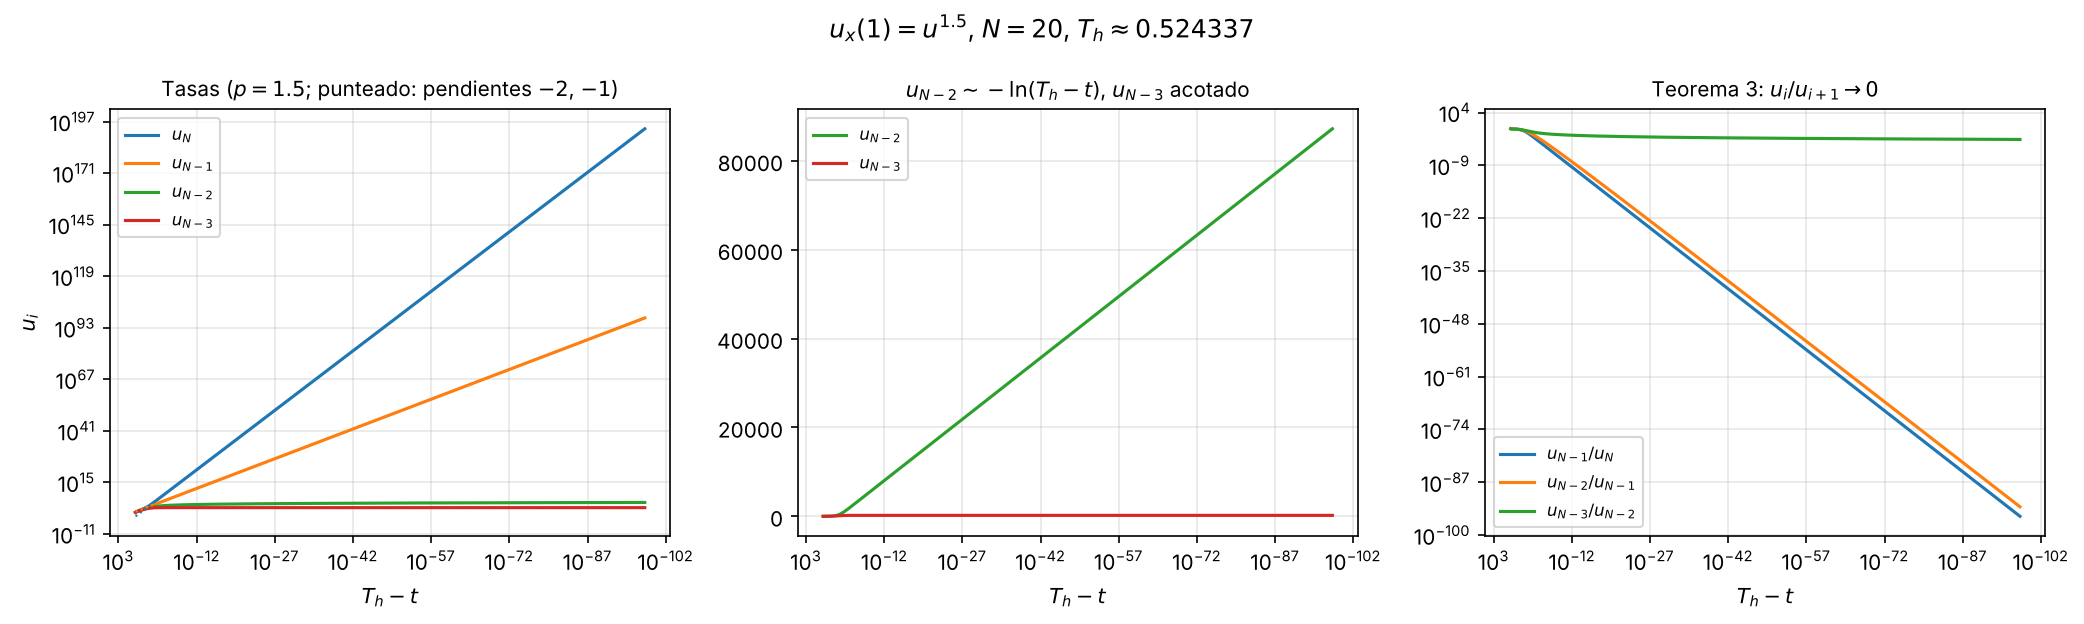
\includegraphics[width=\textwidth]{parabolic/blowup_sets_rates.png}\\[1ex]
\begin{subfigure}{0.48\textwidth}
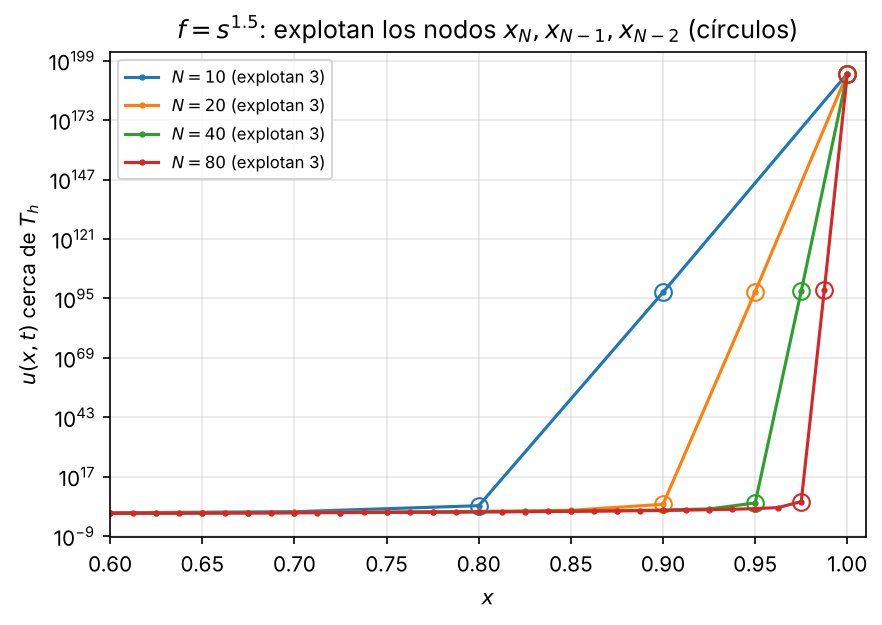
\includegraphics[width=\textwidth]{parabolic/blowup_sets_profiles.png}
\end{subfigure}\hfill
\begin{subfigure}{0.48\textwidth}
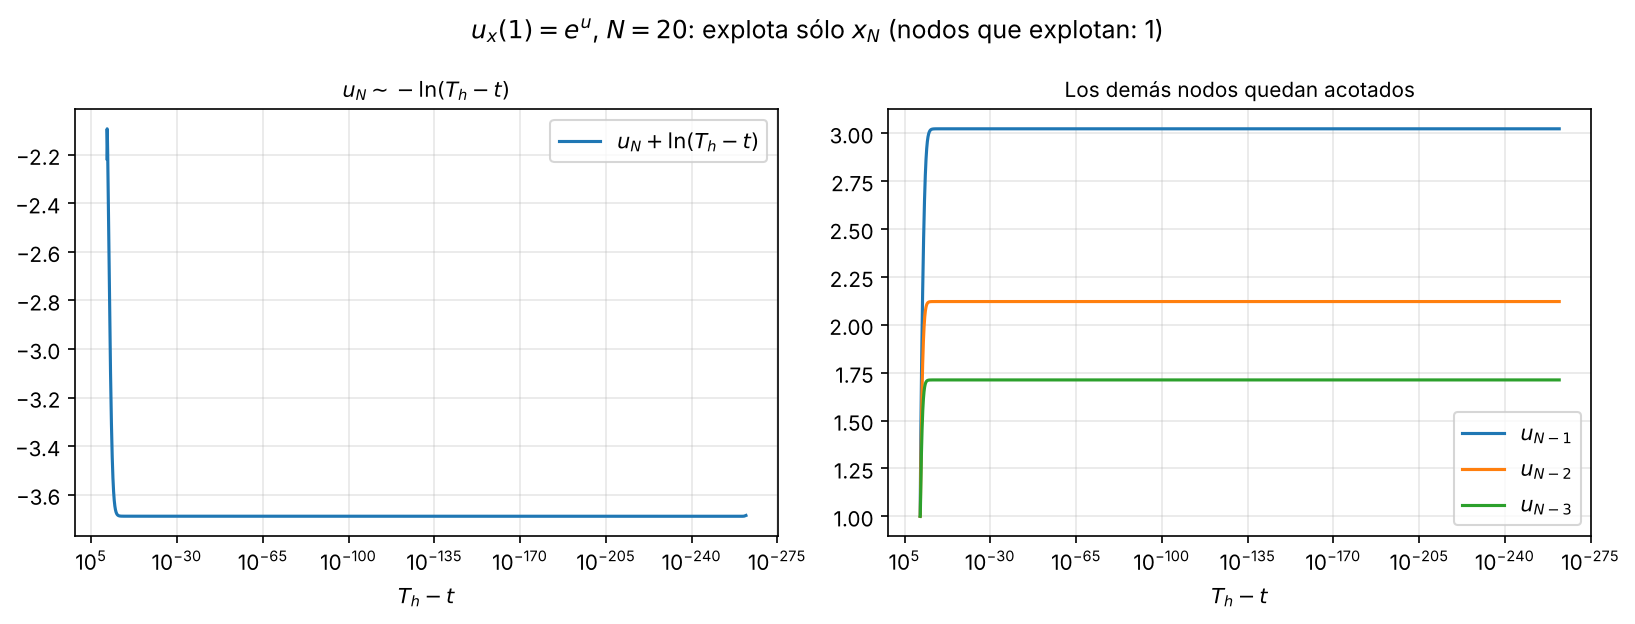
\includegraphics[width=\textwidth]{parabolic/blowup_sets_exp.png}
\end{subfigure}\\[1ex]
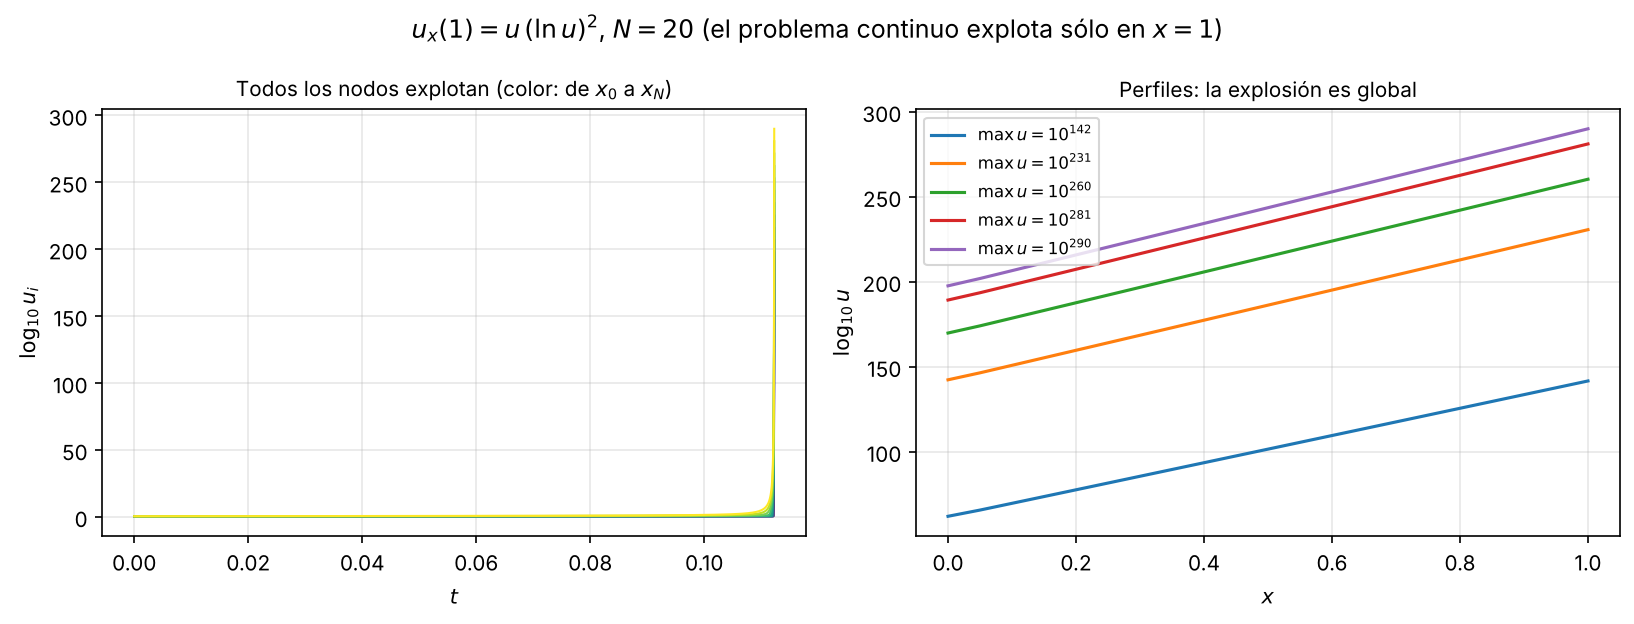
\includegraphics[width=0.8\textwidth]{parabolic/blowup_sets_log.png}
\caption{Conjuntos de blow-up. Arriba: tasas y Teorema~3 para $f=s^{1.5}$.
Centro: perfiles cerca de $T_h$ para varios $N$ (explotan siempre tres
nodos) y el caso $f=e^s$. Abajo: explosión global para $f=s(\ln s)^2$.}
\label{fig:fgr}
\end{figure}

%----------------------------------------------------------------------
\subsection{Estacionarias espurias \cite{FR}}

\paragraph{Problema.} $u_t=u_{xx}-\lambda u^p$, $u_x(0)=0$, $u_x(1)=u^q$.
El continuo explota (para datos grandes) si $p<2q-1$; el semidiscreto sólo
si $p\le q$. Para $q<p<2q-1$ aparece una estacionaria espuria atractiva con
$w_N\approx(2/(\lambda h))^{1/(p-q)}$. Se usa $q=2$, $\lambda=1$. El
artículo es teórico.

\paragraph{Resultados.} La estacionaria espuria se calcula por
\emph{shooting} desde $x=0$ y se refina con Newton; en la recursión se usa
$F_2(w_1)=w_1+\frac{\lambda h^2}{2}w_1^p$ (el artículo imprime
$\lambda h^2$, una errata). Para cada $N$ es la única estacionaria positiva
(el continuo no tiene ninguna), es atractiva y $c_h=w_Nh^{1/(p-q)}\to4$ por
debajo (Tabla~\ref{tab:fr}). Con dato $u_0\equiv3$ el continuo explota; la
solución discreta lo sigue hasta $t\approx0.025$ y luego satura en la
espuria, cada vez más alta al refinar (Figura~\ref{fig:fr}).

\begin{table}[H]
\centering
\begin{tabular}{rccc}
\toprule
$N$ & $w_N$ & $c_h=w_Nh^{1/(p-q)}$ & autovalor máximo\\
\midrule
10 & 382.59 & 3.826 & $-22.98$\\
20 & 1564.27 & 3.911 & $-22.31$\\
40 & 6326.86 & 3.954 & $-21.70$\\
80 & 25450.84 & 3.977 & $-21.31$\\
160 & 102096.93 & 3.988 & $-21.07$\\
\bottomrule
\end{tabular}
\caption{Estacionaria espuria para $p=2.5$, $q=2$, $\lambda=1$.}
\label{tab:fr}
\end{table}

\begin{figure}[H]
\centering
\begin{subfigure}{0.44\textwidth}
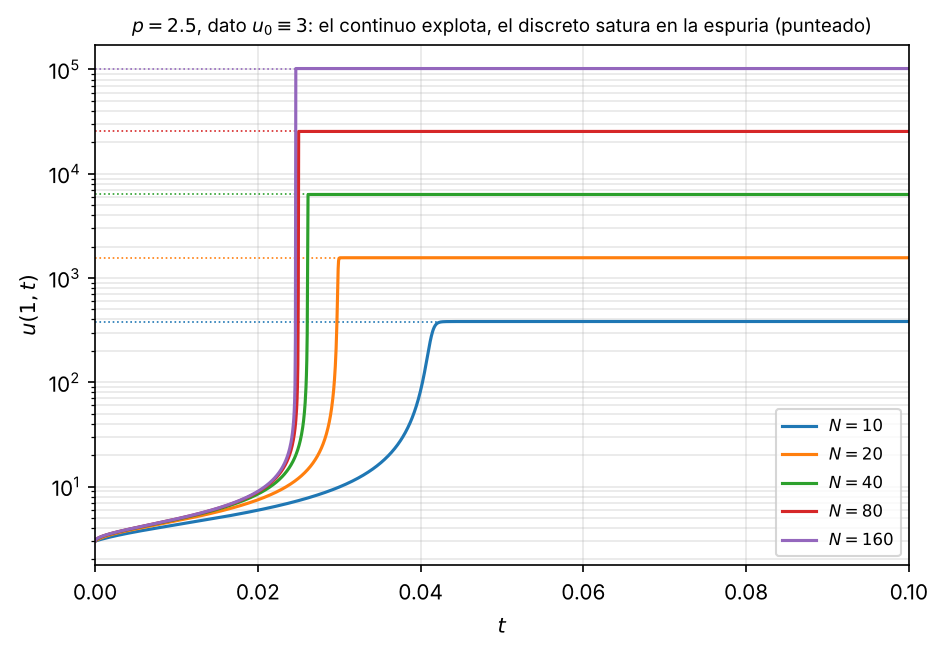
\includegraphics[width=\textwidth]{parabolic/spurious_dynamics.png}
\end{subfigure}\hfill
\begin{subfigure}{0.54\textwidth}
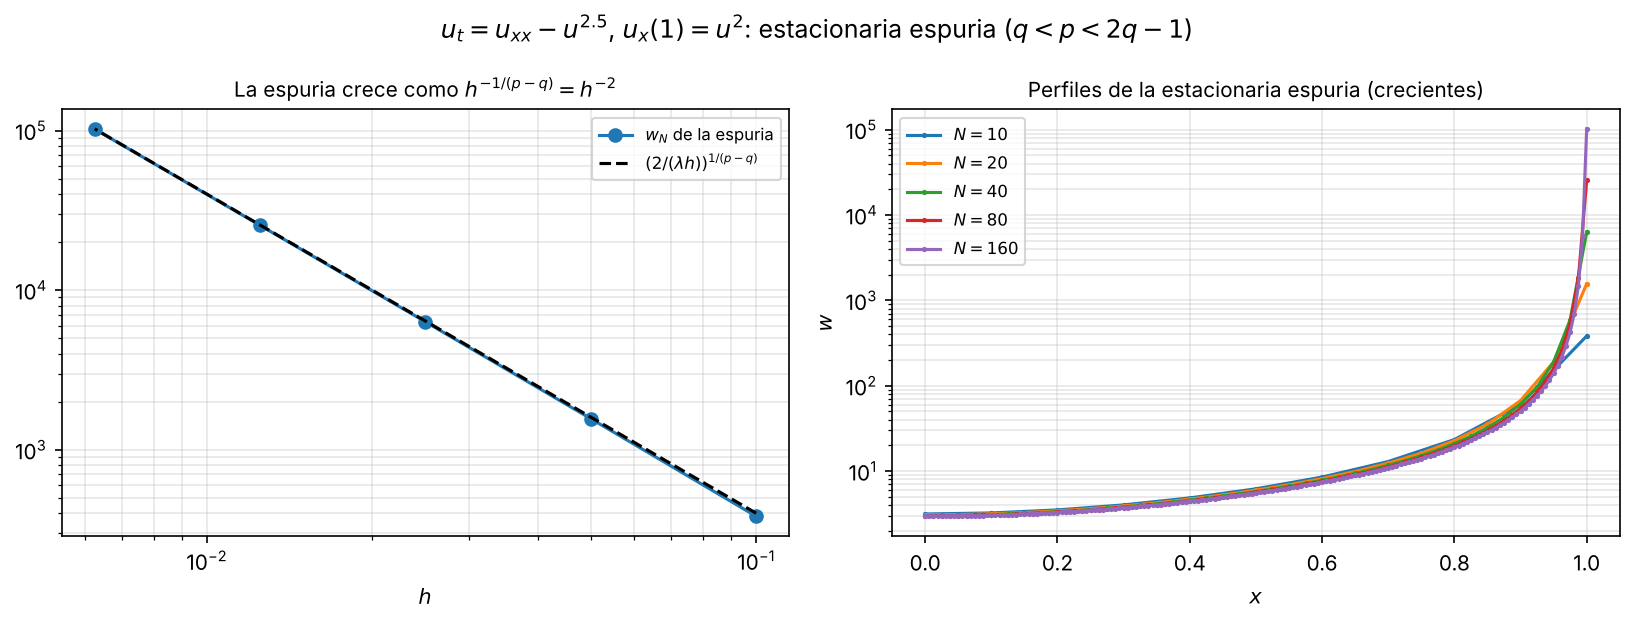
\includegraphics[width=\textwidth]{parabolic/spurious_steady.png}
\end{subfigure}\\[1ex]
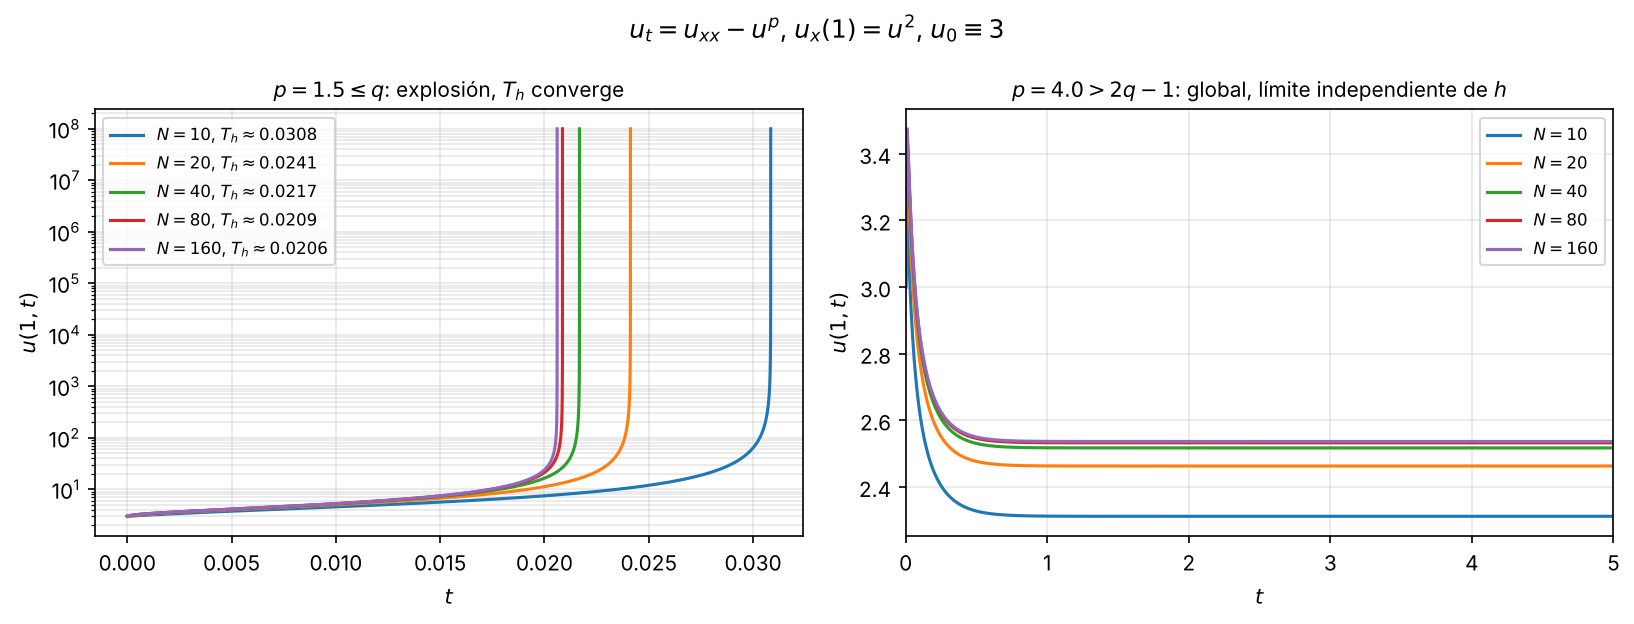
\includegraphics[width=0.85\textwidth]{parabolic/spurious_regimes.png}
\caption{Estacionarias espurias. Arriba: la explosión queda reemplazada por
una estacionaria de tamaño $\sim h^{-2}$. Abajo: para $p=1.5\le q$ el
esquema explota y $T_h$ converge (0.0308, 0.0241, 0.0217, 0.0209, 0.0206);
para $p=4>2q-1$ las soluciones son globales y el límite no depende de $h$.}
\label{fig:fr}
\end{figure}

%----------------------------------------------------------------------
\subsection{Varias dimensiones \cite{AFGR-dims}}

\paragraph{Problema.} $u_t=\Delta u$ en $(0,1)^2$,
$\partial u/\partial\eta=u^p$, con diferencias finitas (Ejemplo~3 de
\cite{AFGR-dims}) escritas como $MU'=-AU+BU^p$, con $A$ simétrica,
$a_{ij}\le0$ fuera de la diagonal y filas de suma nula. Dato
$u_0=1+\frac12(x^2+y^2)$, con máximo en la esquina $(1,1)$. El artículo es
teórico.

\paragraph{Propagación (Teorema 1.5).} El conjunto $F$ de nodos con
$(T_h-t)^{1/(p-1)}u_k\to l_k=(m_k/((p-1)b_k))^{1/(p-1)}$ resulta ser la
esquina en todos los casos, y explotan exactamente los nodos a distancia
$\le K=[1/(p-1)]$ de $F$ en el grafo de $A$, independientemente de $h$
(Tabla~\ref{tab:dims}, Figura~\ref{fig:dims}).

\begin{table}[H]
\centering
\begin{tabular}{ccc}
\toprule
$p$ & $K$ & nodos que explotan ($N=10,20,40$)\\
\midrule
3 & 0 & 1\\
2 & 1 & 3\\
1.8 & 1 & 3\\
1.5 & 2 & 6\\
1.4 & 2 & 6\\
\bottomrule
\end{tabular}
\caption{Propagación del blow-up en el cuadrado.}
\label{tab:dims}
\end{table}

\paragraph{Tasa (Teorema 1.4).} Cerca de $T_h$ la pendiente de
$\log\|U\|_\infty$ contra $\log(T_h-t)$ es exactamente $-1/(p-1)$, distinta
de la continua $-1/(2(p-1))$. Graficada contra $(T_h-t)/h^2$, la pendiente
local de todas las mallas cae sobre una misma curva: el cambio de tasa ocurre
en $T_h-t\approx h^2$. Antes de esa ventana la pendiente se acerca a
$-1/(2(p-1))$ al refinar ($-0.54$ con $N=80$ para $p=2$).

\paragraph{Tiempos (Teorema 1.3).} Para $p=2$, $T_h=0.02794$, $0.02399$,
$0.02282$, $0.02249$, $0.02241$ para $N=10,\dots,160$; el orden observado
tiende a $2$ ($1.75$, $1.86$, $1.91$) y por Richardson $T\approx0.02238$.

\begin{figure}[H]
\centering
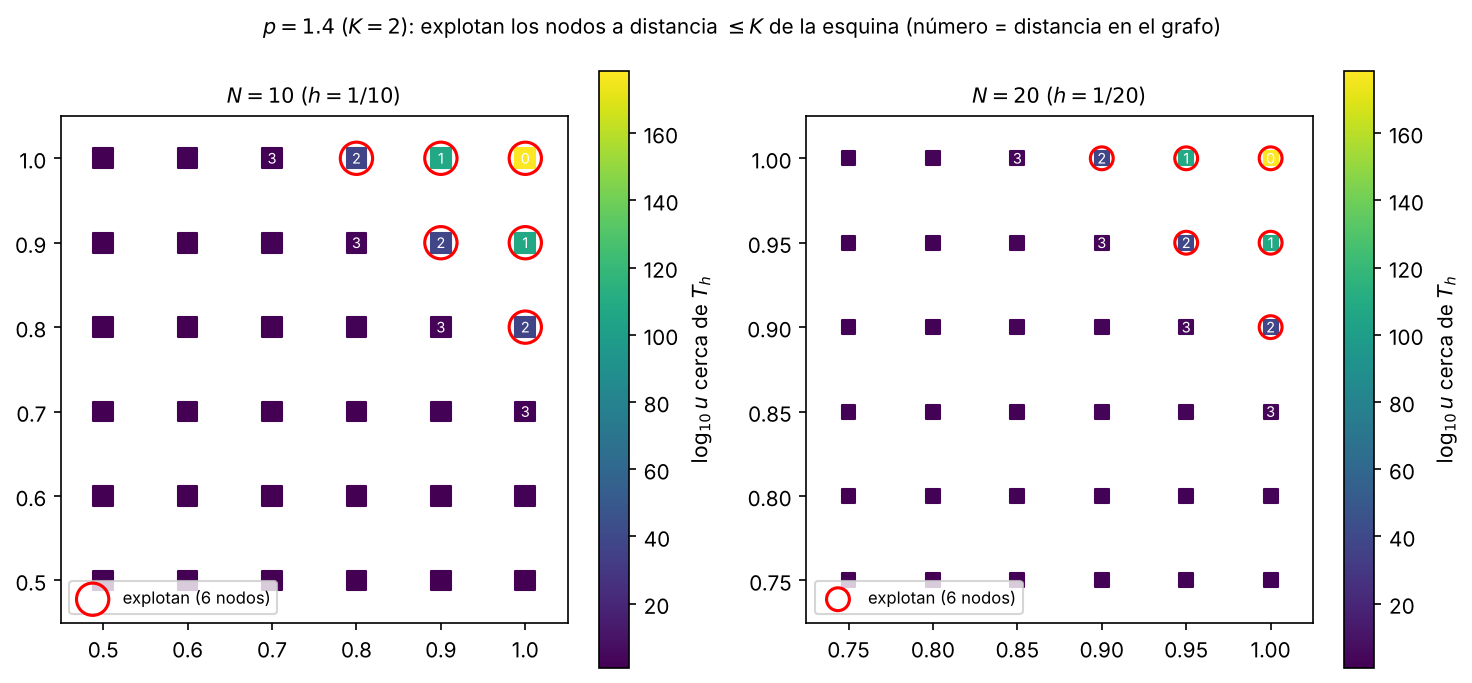
\includegraphics[width=0.85\textwidth]{parabolic/several_dims_propagation.png}\\[1ex]
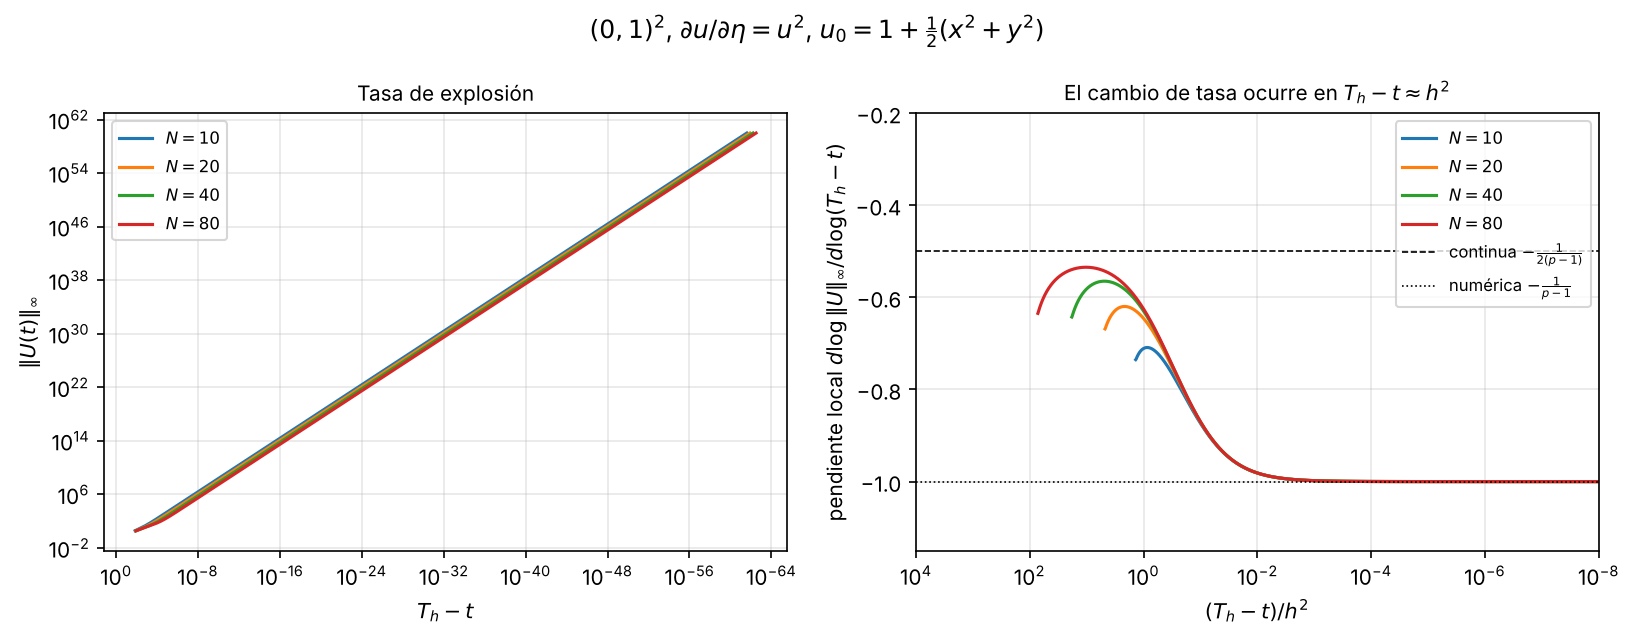
\includegraphics[width=0.95\textwidth]{parabolic/several_dims_rate.png}
\caption{Varias dimensiones. Arriba: nodos que explotan para $p=1.4$ ($K=2$);
el número indica la distancia en el grafo a la esquina. Abajo: tasa de
explosión y cambio de pendiente en $T_h-t\approx h^2$.}
\label{fig:dims}
\end{figure}

%----------------------------------------------------------------------
\subsection{Sistema: blow-up simultáneo y no simultáneo \cite{AFGR-sys}}

\paragraph{Problema.} $u_t=u_{xx}$, $v_t=v_{xx}$ en $(0,1)$ con
$\partial_\eta u=u^{p_{11}}v^{p_{12}}$, $\partial_\eta v=u^{p_{21}}v^{p_{22}}$
en $x=0,1$. Para sistemas se usa la regla de reescalamiento genérica
$dt/ds=\min(1,\|Y\|_\infty/\|Y'\|_\infty)$. El artículo es teórico.

\paragraph{Existencia (Teorema 1.2).} En la familia $p_{11}=p_{22}=a$,
$p_{12}=p_{21}=b$, con una grilla de $15\times15$ y dato asimétrico
$(U_0,V_0)=(2,0.5)$, los $225$ puntos coinciden con el teorema: hay explosión
si y sólo si $a>1$ o $(a-1)^2<b^2$. Para decidir se comparan los tiempos que
tarda $\|Y\|_\infty$ en pasar de $10^{30}$ a $10^{60}$ y de $10^{60}$ a
$10^{90}$: el cociente es menor que $1$ si hay explosión, $1$ si el
crecimiento es exponencial y enorme si es polinomial.

\paragraph{No simultaneidad (Teoremas 1.4--1.5).} Con $p_{11}=3$,
$p_{12}=1$, $p_{22}=0$ y dato $(2,1)$, $V$ queda acotada si y sólo si
$p_{21}<p_{11}-1=2$: acotada para $p_{21}\in\{0,1,1.5\}$, explota para
$p_{21}\in\{2.5,3,4\}$, para $N=10,20,40,80$. En el caso no simultáneo,
$\|U\|_\infty\sim(T_h-t)^{-1/(p_{11}-1)}$ (Figura~\ref{fig:sys}).

\begin{figure}[H]
\centering
\begin{subfigure}{0.38\textwidth}
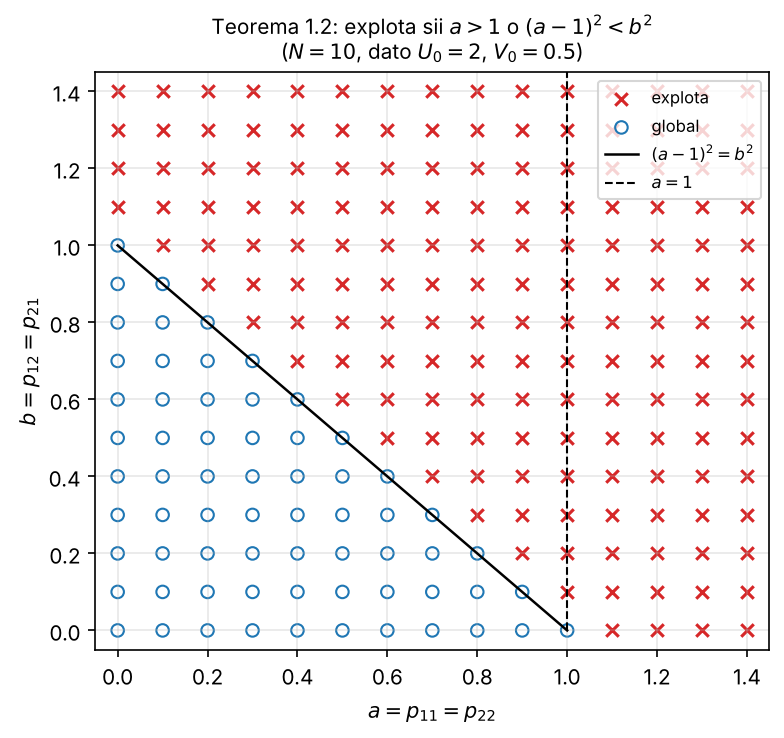
\includegraphics[width=\textwidth]{parabolic/system_existence.png}
\end{subfigure}\hfill
\begin{subfigure}{0.6\textwidth}
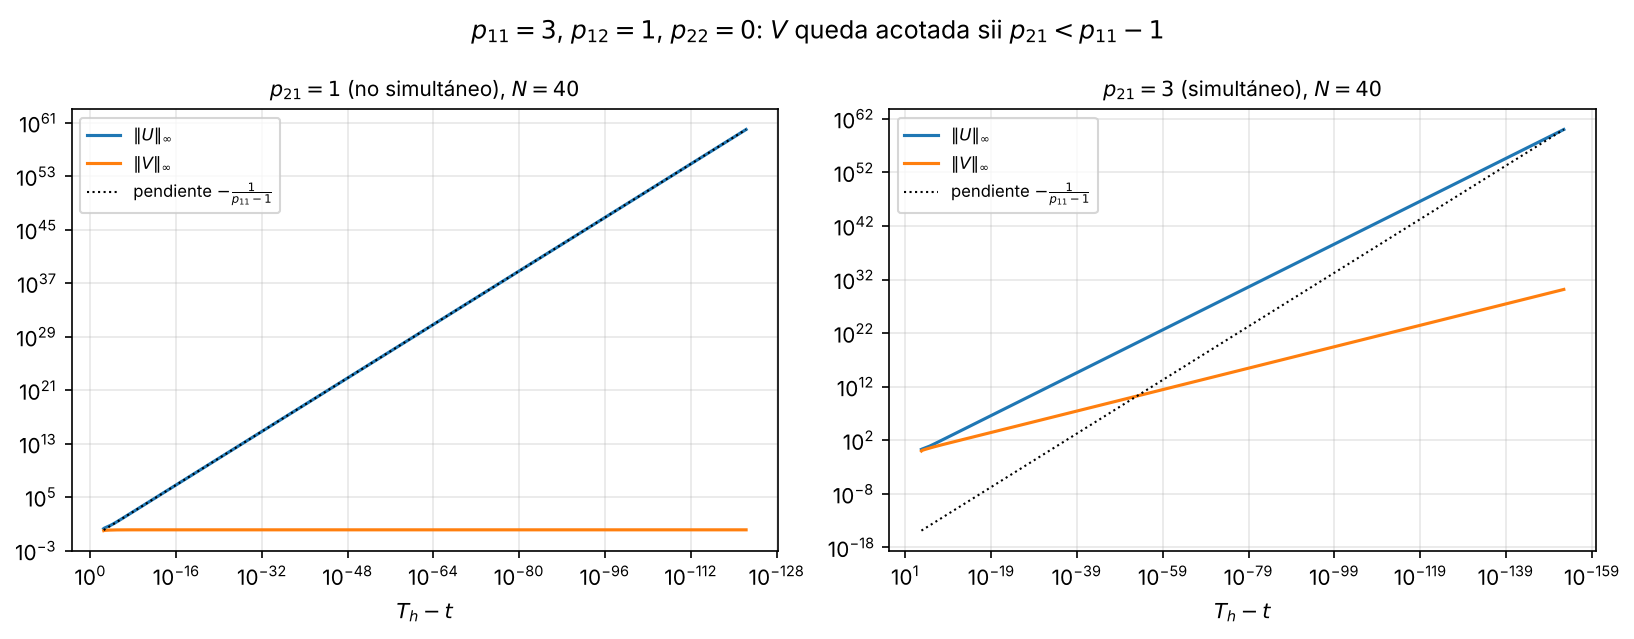
\includegraphics[width=\textwidth]{parabolic/system_nonsimultaneous.png}
\end{subfigure}
\caption{Sistema. Izquierda: diagrama de existencia de blow-up. Derecha:
blow-up no simultáneo ($p_{21}=1$) y simultáneo ($p_{21}=3$).}
\label{fig:sys}
\end{figure}

%======================================================================
\section{Ecuaciones estocásticas}\label{sec:estoc}

\subsection{EDEs con explosión \cite{DFGRS}}

\paragraph{Esquema.} Para $dx=b(x)\,dt+\sigma(x)\,dW$, Euler--Maruyama con
paso $\tau_k=h/b(X_k)$, de modo que la deriva avanza exactamente $h$ por
paso; el algoritmo se detiene cuando $|X_k|\ge M$ y $R_h^M=t_k$ aproxima el
tiempo de explosión. Experimentos del artículo:
$b(\xi)=|\xi|^{1.1}+0.1$, $\sigma=\sqrt b$, $z=10$.

\paragraph{Valores elegidos.} El artículo no da $h$ ni $M$ en algunas
figuras. Se usó $h=0.25$ en las Figuras~1 y~2 (da $\approx4\times10^5$
pasos, el rango del eje de la Figura~2) y $M=10^4$ en la Figura~3 (con
$M=10^5$ la densidad quedaría centrada en $\approx4.8$ y no en $\approx4.0$
como en el original). La leyenda de la Figura~3 dice $h=0.01$, pero el texto
y $\tau_1\simeq0.008$ corresponden a $h=0.1$.

\paragraph{Resultados.} Las tres figuras se reproducen (Figura~\ref{fig:sde}).
En la Figura~3, con 1000 trayectorias por valor de $h$, las medias de
$R_h^M$ son $4.032$, $4.020$, $4.006$ para $h=1,0.5,0.1$ (desvíos
$\approx0.24$). Para estos $M$, $R_h^M$ todavía está lejos del verdadero
tiempo de explosión: la cola determinista $\int_M^\infty ds/b\approx10M^{-0.1}$
vale $\approx4$ para $M=10^4$; la convergencia en $M$ es muy lenta porque
$b\sim s^{1.1}$.

\begin{figure}[H]
\centering
\begin{subfigure}{0.48\textwidth}
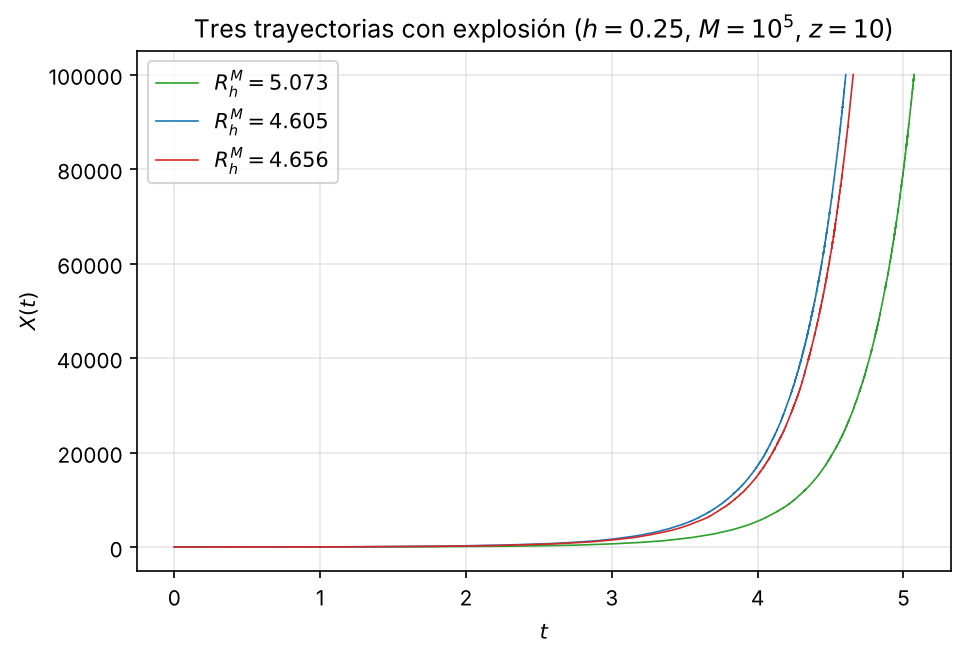
\includegraphics[width=\textwidth]{sode/fig1_paths.png}
\caption{Figura 1: tres trayectorias, $M=10^5$.}
\end{subfigure}\hfill
\begin{subfigure}{0.48\textwidth}
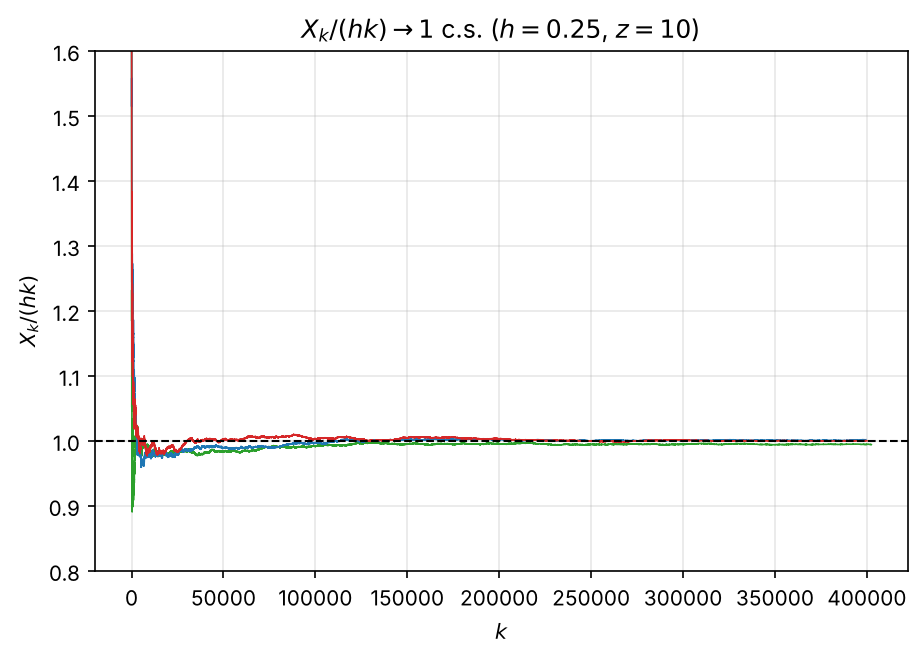
\includegraphics[width=\textwidth]{sode/fig2_ratio.png}
\caption{Figura 2: $X_k/(hk)\to1$.}
\end{subfigure}\\[1ex]
\begin{subfigure}{0.55\textwidth}
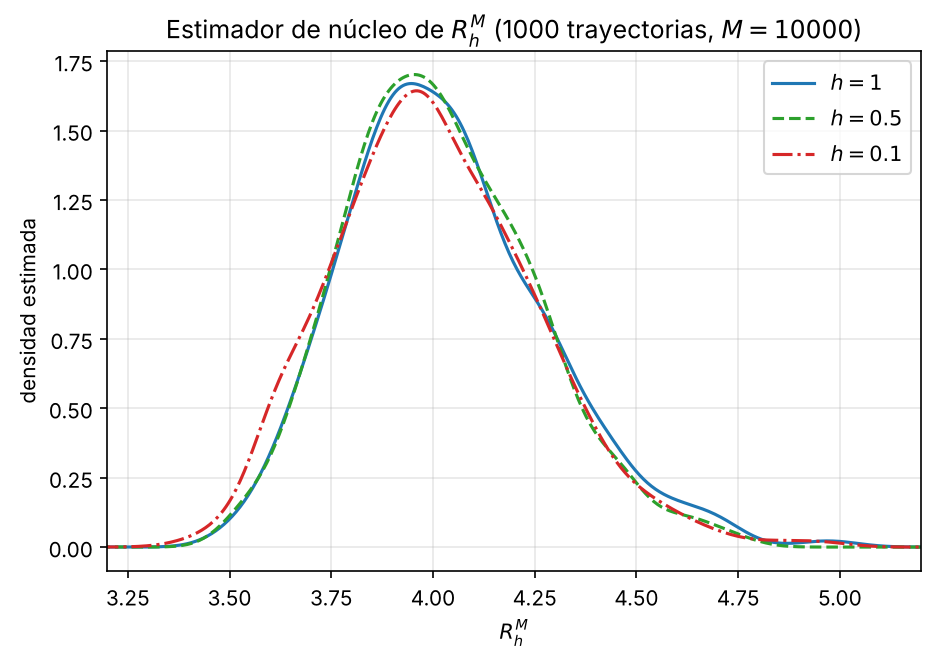
\includegraphics[width=\textwidth]{sode/fig3_kde.png}
\caption{Figura 3: densidad de $R_h^M$.}
\end{subfigure}
\caption{EDEs con explosión.}
\label{fig:sde}
\end{figure}

%----------------------------------------------------------------------
\subsection{Ruido blanco espacio-temporal \cite{FG}}

\paragraph{Esquema.} $u_t=u_{xx}+(u_+)^2+\sigma\dot W$ en $(0,1)$ con
Dirichlet homogéneo, $u_0\equiv0$, $h=0.02$; diferencias finitas en espacio,
ruido $\sigma\sqrt{\tau_j/h}\,\xi_k$ por paso y Euler explícito con paso
$\tau_j=\min(\tau_{\max},\tau/\|u^j\|_{L^1})$, $\tau=5\cdot10^{-4}$,
$\tau_{\max}=0.4h^2$; explosión cuando $\max u\ge10^{13}$. El artículo no
da $\tau$ ni dice qué hacer cuando $\sum_kh\,u_k\le0$ (pasa en $t=0$); se
agregó el valor absoluto y la cota $\tau_{\max}$. La escala del ruido elegida
es la coherente con la prueba del Teorema~4.1 y reproduce la amplitud de las
fluctuaciones de la Figura~1 original.

\paragraph{Resultados.} Las Figuras~1--3 y la Tabla~1 se reproducen
cualitativamente (Figura~\ref{fig:spde}): la trayectoria explota en
$t\approx69.94$ (en el artículo, $72.51$), con máximos $5.0$ en $t=1$ y $3.7$
en $t=50$ (contra $5.6$ y $3.4$). Para $\sigma\le5$ no hay explosiones hasta
$t=1000$, como en el artículo. En la Figura~4, con 832 trayectorias, se
obtiene media $94.0$ y desvío $94.9$, contra $46.9$ y $43.9$ en el artículo:
el tiempo medio da el doble (ver Sección~\ref{sec:discrepancias}). Lo
cualitativo coincide: media $\approx$ desvío y densidad de forma
exponencial.

\begin{figure}[H]
\centering
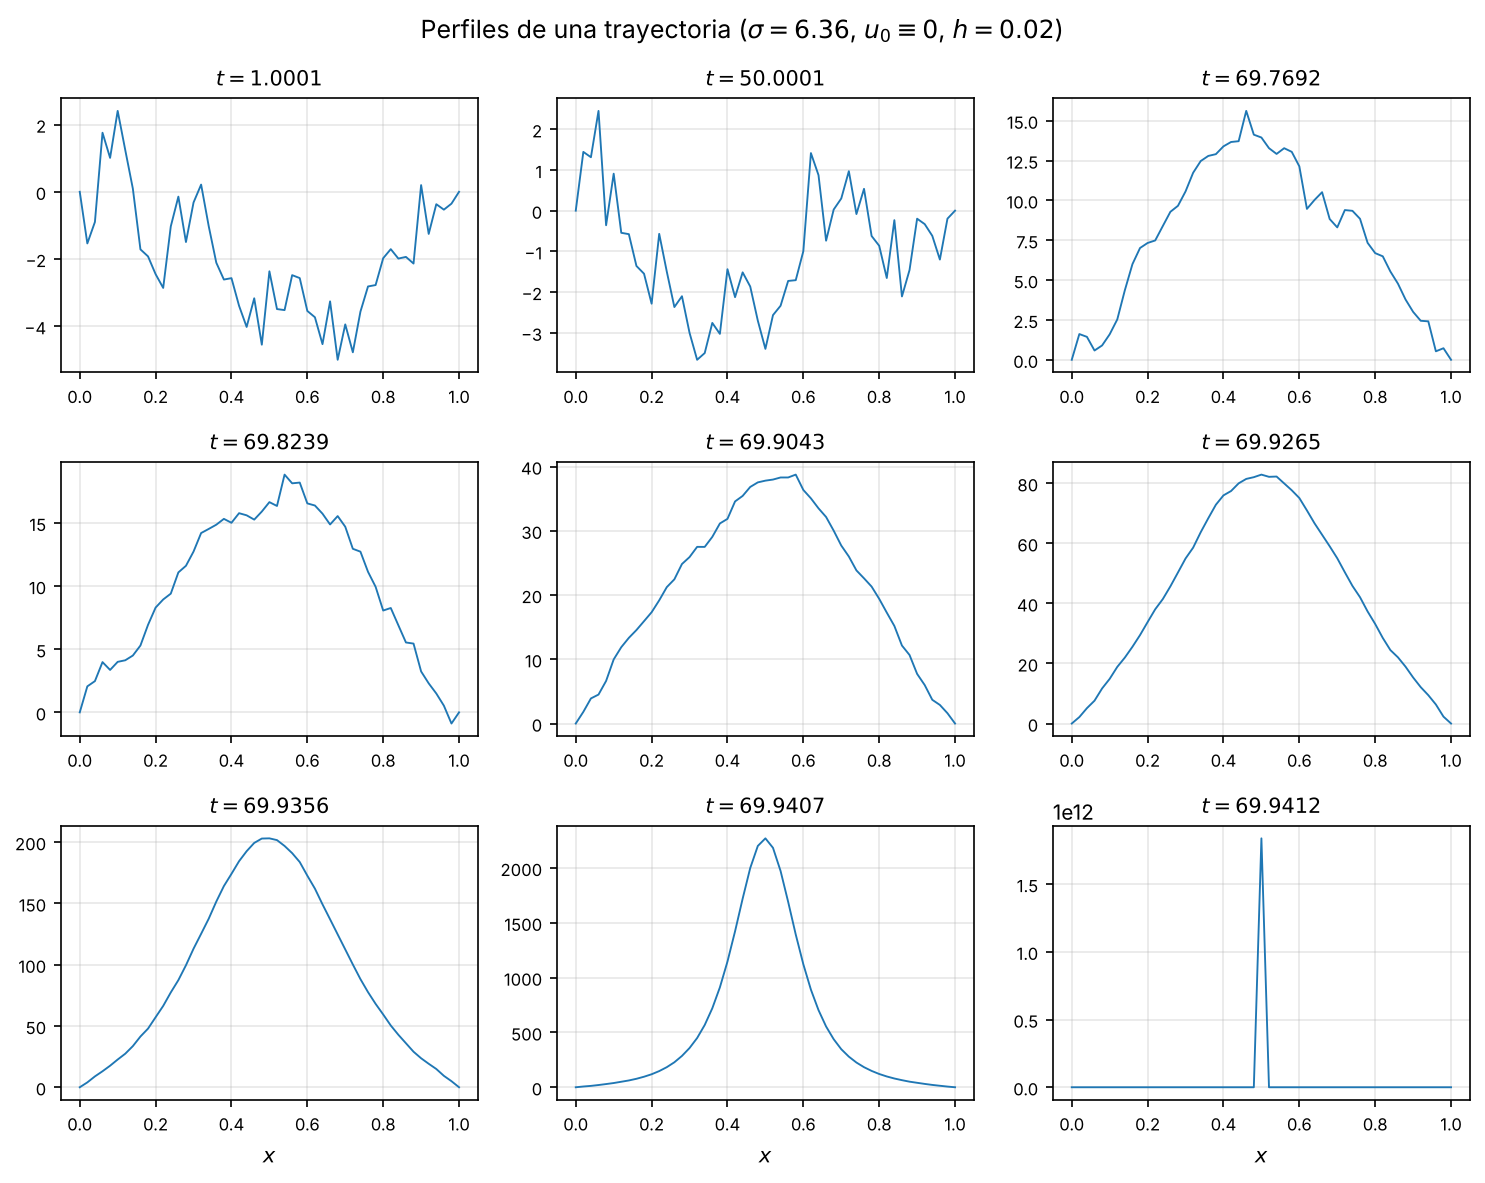
\includegraphics[width=0.8\textwidth]{spde/fig1_profiles.png}\\[1ex]
\begin{subfigure}{0.5\textwidth}
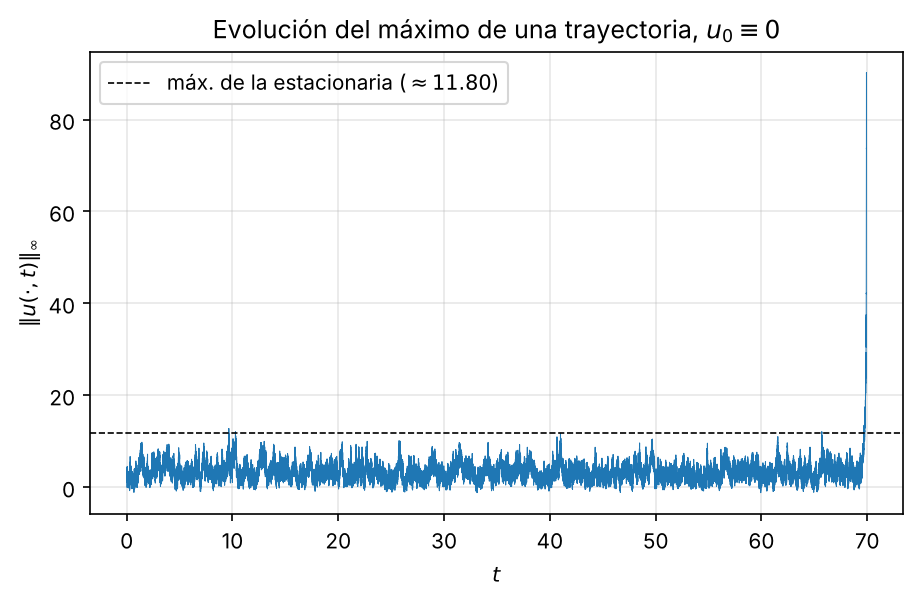
\includegraphics[width=\textwidth]{spde/fig2_max.png}
\end{subfigure}\hfill
\begin{subfigure}{0.42\textwidth}
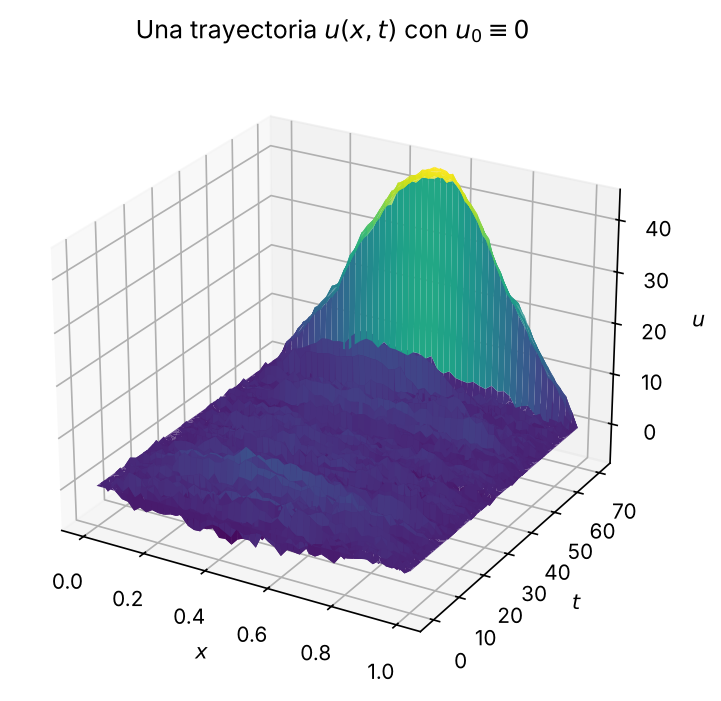
\includegraphics[width=\textwidth]{spde/fig3_surface.png}
\end{subfigure}\\[1ex]
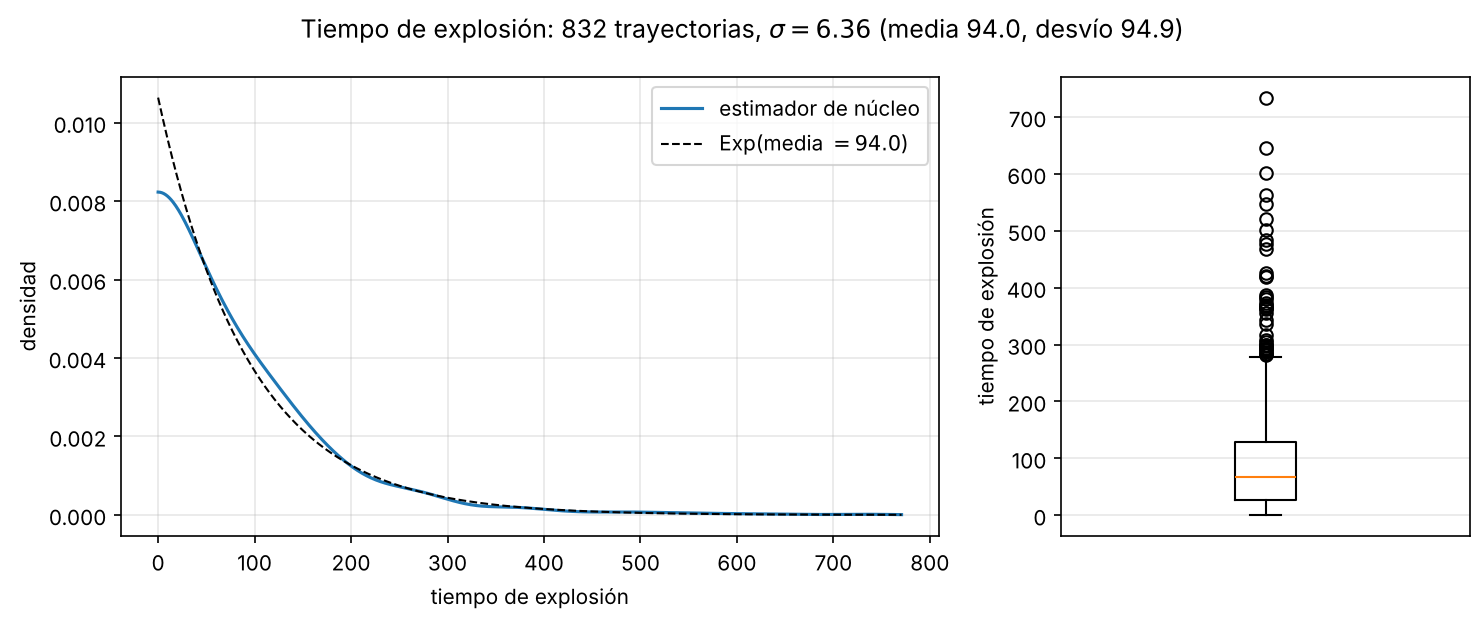
\includegraphics[width=0.85\textwidth]{spde/fig4_explosion_time.png}
\caption{SPDE con ruido blanco: Figuras 1--4 de \cite{FG}.}
\label{fig:spde}
\end{figure}

\paragraph{Experimento nuevo: ley exponencial.} El artículo conjetura que
$T_\sigma/\mathbb E(T_\sigma)$ converge a una exponencial de media $1$
cuando $\sigma\to0$, problema estudiado luego en
\cite{GS,GSS}. Se compararon $T/\bar T$ y Exp(1) con 832 trayectorias por
valor de $\sigma$ (Tabla~\ref{tab:exp}, Figura~\ref{fig:exp}); el p-valor de
Kolmogorov--Smirnov se calcula por Monte Carlo porque la media se estima.
Para $\sigma\le7$ no se rechaza la exponencialidad; para $\sigma$ grande la
explosión deja de ser un evento raro y la ley se aparta de la exponencial
(cola más liviana, tiempo mínimo de tránsito). El experimento con
$\sigma\le5$ confirma el comportamiento metaestable.

\begin{table}[H]
\centering
\begin{tabular}{ccccc}
\toprule
$\sigma$ & media & desvío/media & estadístico KS & p-valor\\
\midrule
6.36 & 94.01 & 1.01 & 0.031 & 0.18\\
7 & 36.52 & 0.98 & 0.021 & 0.68\\
8 & 13.57 & 1.00 & 0.044 & 0.006\\
10 & 4.43 & 0.89 & 0.074 & $<0.001$\\
\bottomrule
\end{tabular}
\caption{Tiempo de explosión normalizado contra Exp(1).}
\label{tab:exp}
\end{table}

\begin{figure}[H]
\centering
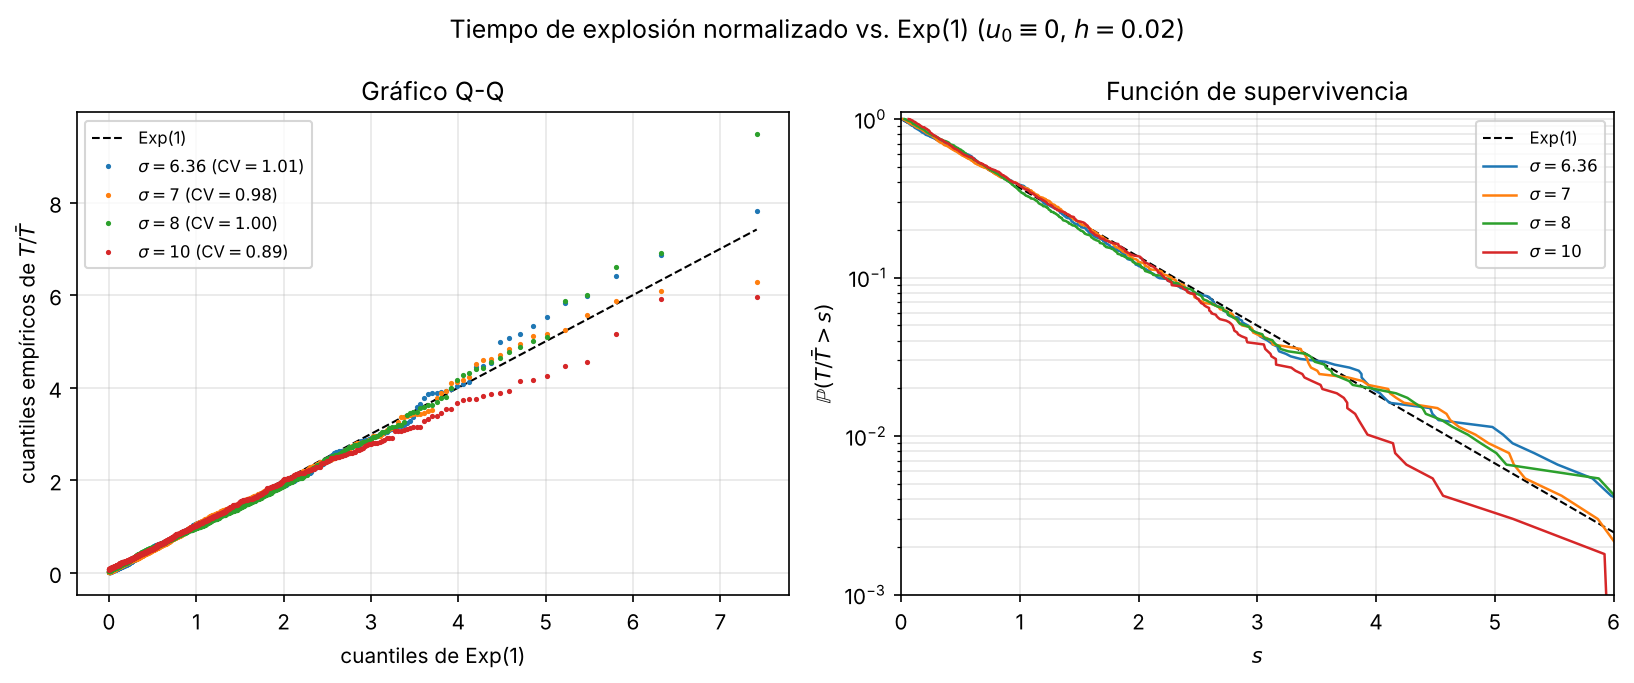
\includegraphics[width=0.95\textwidth]{spde/exponential_law.png}\\[1ex]
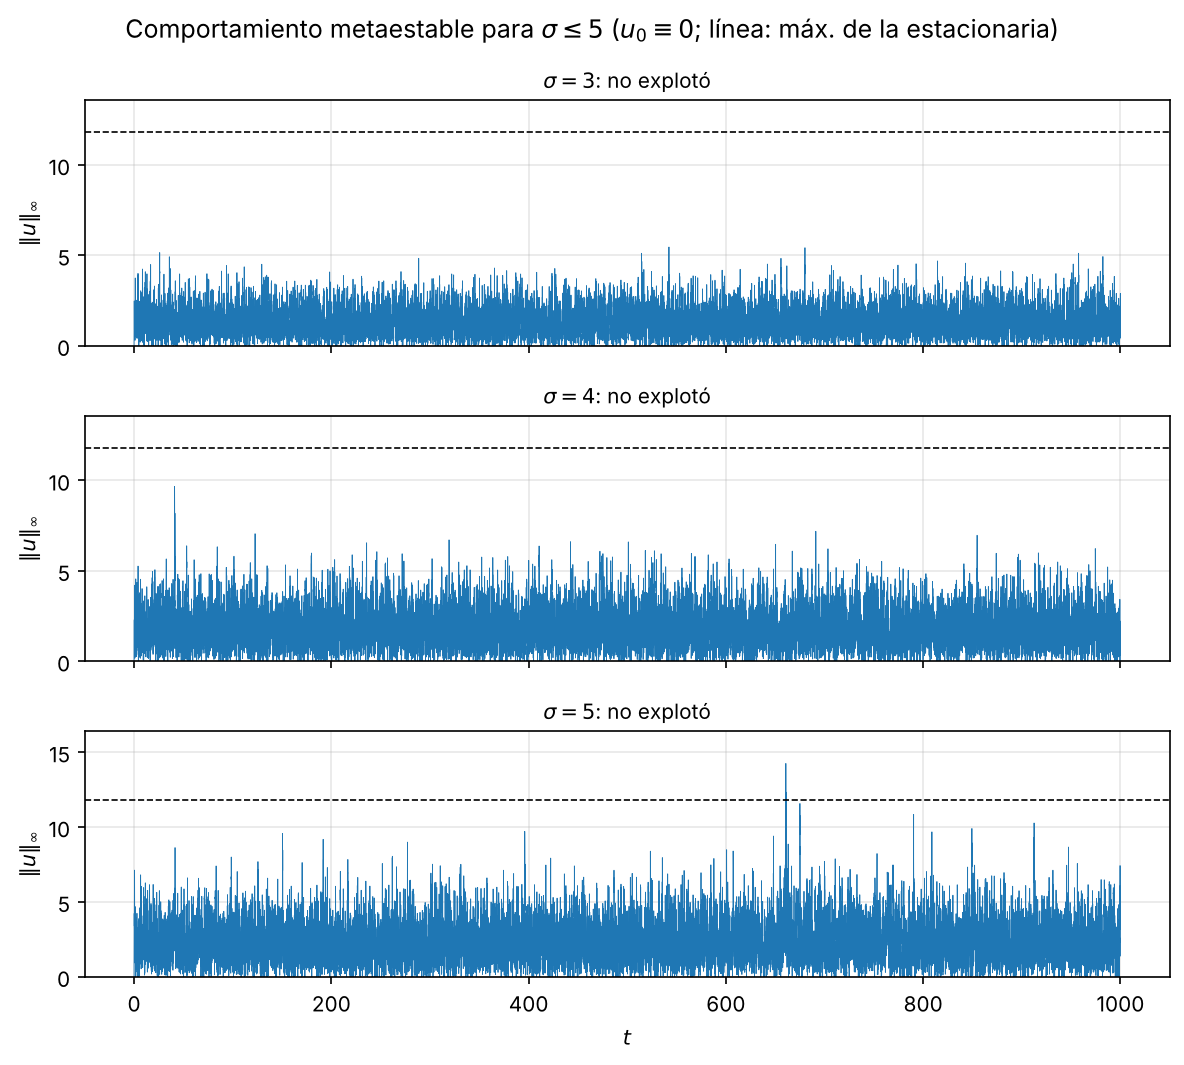
\includegraphics[width=0.6\textwidth]{spde/exp0_metastable.png}
\caption{Arriba: gráfico Q-Q y función de supervivencia de $T/\bar T$.
Abajo: metaestabilidad para $\sigma\le5$ (sin explosiones hasta $t=1000$).}
\label{fig:exp}
\end{figure}

%======================================================================
\section{Paso temporal adaptativo}\label{sec:adapt}

El paquete \code{blowup.adaptive} implementa la regla de paso de los
artículos,
\[
\tau_n=\frac{\tau}{\max\big(1,\psi(U_n)\big)},\qquad T_\tau=\sum_{n\ge0}\tau_n,
\]
para cualquier sistema $U'=F(U)$, con varias elecciones de $\psi$:
$\|U\|_\infty^{p-1}$ (regla clásica $\tau\min(1,\|U_n\|^{1-p})$),
$f(m)/m$, $b(X)$ (la regla $h/b(X_k)$ de \cite{DFGRS}), $\|u\|_{L^1}$ (la
regla de \cite{FG}) y una genérica $\|U'\|/\|U\|$ que no requiere conocer la
no linealidad. Hay dos variantes:
\begin{itemize}
\item \textbf{Totalmente discreta}: Euler explícito, IMEX
$(I-\tau_nL)U_{n+1}=U_n+\tau_nN(U_n)$ (parte lineal implícita, no lineal
explícita) y Euler implícito con Newton. El tiempo restante $T_\tau-t_n$ se
calcula sumando los pasos posteriores, sin cancelación.
\item \textbf{Continua}: el reescalamiento de la Sección~\ref{sec:rescaling}
con un integrador de alto orden.
\end{itemize}

\paragraph{Validación.} Para $u'=u^2$, $u(0)=1$ ($T=1$), Euler explícito
con $\tau_n=\tau/u_n$ da $T_\tau=1+\tau$ exactamente, y el implícito
converge con orden~1. Con paso fijo la solución discreta está definida para
todo $n$ y crece doblemente exponencial en $n$: llega a $10^{150}$ en
$t=1.6$, cuando el verdadero tiempo de explosión es $1$. Para
$u_x(1)=u^2$ con $N=20$, $T_\tau\to T_h$ con orden~1 (explícito $1.00$,
IMEX $0.84$ todavía preasintótico, implícito $1.06$), y el esquema discreto
reproduce la tasa $u_N\sim(T_\tau-t_n)^{-1}$ (pendiente medida $-1.0000$) y
la explosión de exactamente dos nodos (Figura~\ref{fig:adapt}).

\begin{figure}[H]
\centering
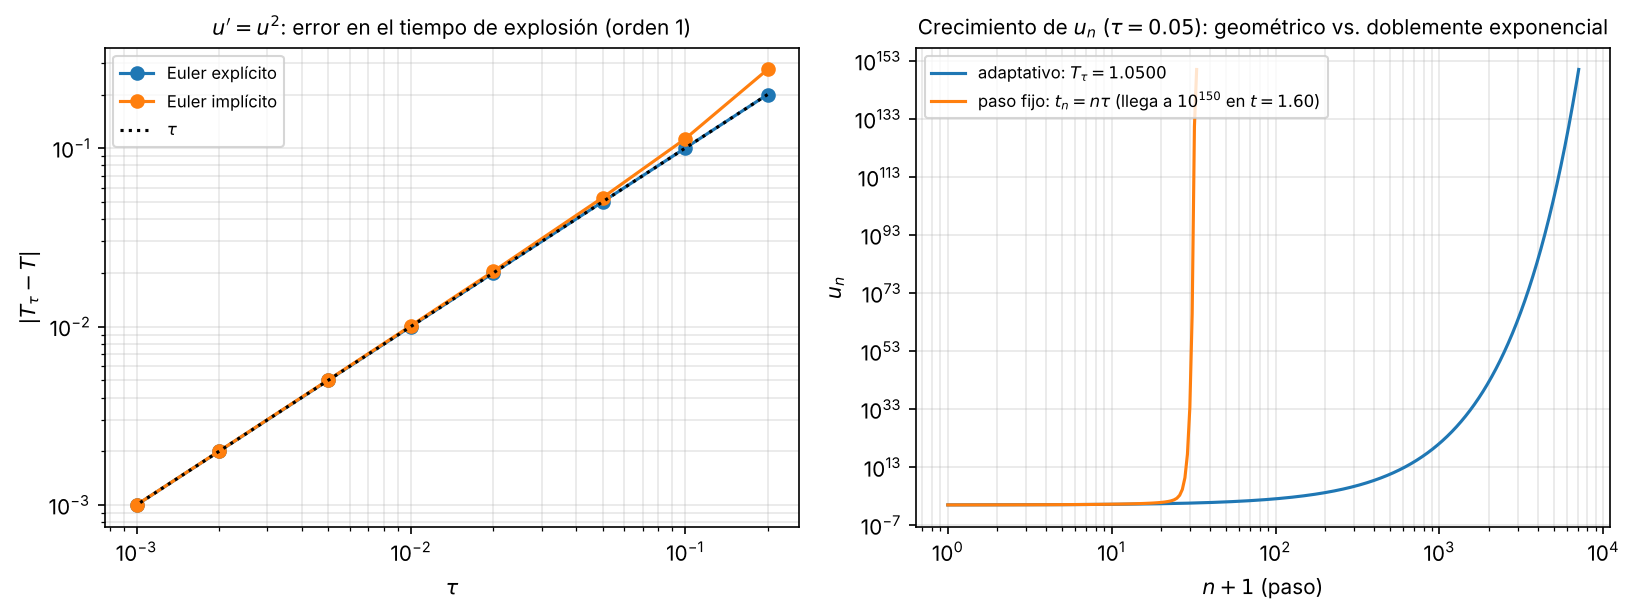
\includegraphics[width=0.95\textwidth]{adaptive/discrete_ode.png}\\[1ex]
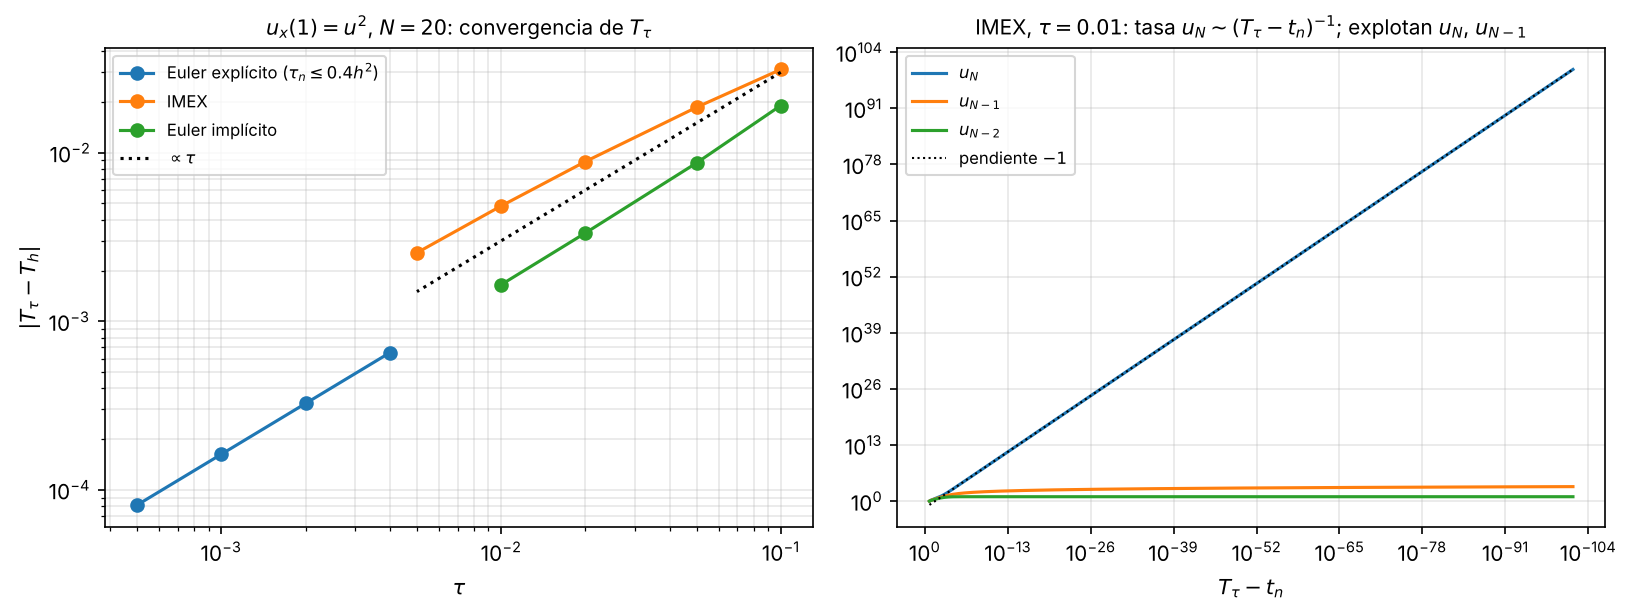
\includegraphics[width=0.95\textwidth]{adaptive/discrete_pde.png}
\caption{Validación del paso adaptativo. Arriba: $u'=u^2$. Abajo:
$u_x(1)=u^2$, $N=20$.}
\label{fig:adapt}
\end{figure}

%======================================================================
\section{Discrepancias, erratas y cuestiones abiertas}\label{sec:discrepancias}

\begin{itemize}
\item \textbf{Tabla 1 de \cite{AFR} para $N$ chico.} Para $N=10$ y $N=20$
los valores de $\lambda_{c,h}$ difieren en $\sim10^{-3}$ de los publicados;
para $N=50$ y $N=100$ coinciden. No se identificó la causa.
\item \textbf{Tiempo medio de explosión en \cite{FG}.} Da $94.0$ contra
$46.9$. No depende del paso temporal (con $100$ trayectorias da $\approx104$
para $\tau_{\max}=0.1h^2$, $0.25h^2$ y $0.49h^2$). Como el tiempo depende
exponencialmente de $1/\sigma^2$, la diferencia equivale a un error de
$\sim7\%$ en la intensidad efectiva del ruido ($\sigma=7$ da media $36.5$).
Probablemente viene de una convención no especificada del código original
(celda del ruido, indexación de la malla o tratamiento de $\sum_khu_k\le0$).
\item \textbf{$K$ contra $K+1$ en \cite{FGR}.} El texto dice que explotan
exactamente $K=[1/(p-1)]$ nodos; los experimentos y las fórmulas del
artículo dan $K+1$.
\item \textbf{Erratas.} En \cite{FR}, $F_2(w_1)$ debe ser
$w_1+\frac{\lambda h^2}{2}w_1^p$. En \cite{AFGR-sys}, el abstract dice
$p_{21}<2(p_{11}-1)$ y los teoremas $p_{21}<p_{11}-1$ (lo correcto, según
los experimentos). En \cite{DFGRS}, la leyenda de la Figura~3 dice $h=0.01$
y debería decir $h=0.1$.
\end{itemize}

%======================================================================
\section{Reproducibilidad}\label{sec:repro}

Requiere Python $\ge3.10$ con NumPy, SciPy y Matplotlib
(\code{pip install -r requirements.txt}). Desde la raíz del repositorio:

\begin{center}
\small
\begin{tabular}{ll}
\toprule
Script & Resultados\\
\midrule
\code{experiments.parabolic.stable\_manifold\_table1} & Tabla~\ref{tab:afr}\\
\code{experiments.parabolic.stable\_manifold\_fig1} & Figura~\ref{fig:afr}\\
\code{experiments.parabolic.stable\_manifold\_slice} & Figura~\ref{fig:slice}\\
\code{experiments.parabolic.dirichlet\_threshold} & Tabla~\ref{tab:dir}, Figura~\ref{fig:dir}\\
\code{experiments.parabolic.blowup\_sets} & Tabla~\ref{tab:fgr}, Figura~\ref{fig:fgr}\\
\code{experiments.parabolic.spurious} & Tabla~\ref{tab:fr}, Figura~\ref{fig:fr}\\
\code{experiments.parabolic.several\_dims} & Tabla~\ref{tab:dims}, Figura~\ref{fig:dims}\\
\code{experiments.parabolic.system} & Figura~\ref{fig:sys}\\
\code{experiments.sode.fig1\_paths}, \code{fig2\_ratio}, \code{fig3\_kde} & Figura~\ref{fig:sde}\\
\code{experiments.spde.fig1\_3\_sample\_path}, \code{fig4\_explosion\_time} & Figura~\ref{fig:spde}\\
\code{experiments.spde.exponential\_law}, \code{exp0\_metastable} & Tabla~\ref{tab:exp}, Figura~\ref{fig:exp}\\
\code{experiments.adaptive.discrete} & Figura~\ref{fig:adapt}\\
\bottomrule
\end{tabular}
\end{center}
Cada script se corre como \code{python -m <script>}. Los tiempos de
explosión de la SPDE se guardan en \code{results/spde/} y se reutilizan. Los
tests se corren con \code{python -m pytest}.

%======================================================================
\begin{thebibliography}{99}
\bibitem{AFR} G. Acosta, J. Fernández Bonder and J.D. Rossi. Stable manifold
approximation for the heat equation with nonlinear boundary conditions.
\emph{J. Dynam. Differential Equations}, 12 (2000), no. 3, 557--578.
\bibitem{FR} J. Fernández Bonder and J.D. Rossi. Blow-up vs. spurious steady
solutions. \emph{Proc. Amer. Math. Soc.}, 129 (2001), no. 1, 139--144.
\bibitem{FGR} J. Fernández Bonder, P. Groisman and J.D. Rossi. On numerical
blow-up sets. \emph{Proc. Amer. Math. Soc.}, 130 (2002), no. 7, 2049--2055.
\bibitem{AFGR-dims} G. Acosta, J. Fernández Bonder, P. Groisman and J.D.
Rossi. Numerical approximation of a parabolic problem with a nonlinear
boundary condition in several space dimensions. \emph{Discrete Contin.
Dynam. Systems - Series B}, 2 (2002), no. 2, 279--294.
\bibitem{AFGR-sys} G. Acosta, J. Fernández Bonder, P. Groisman and J.D.
Rossi. Simultaneous vs. non-simultaneous blow-up in numerical approximations
of a parabolic system with nonlinear boundary conditions. \emph{M2AN Math.
Model. Numer. Anal.}, 36 (2002), no. 1, 55--68.
\bibitem{DFGRS} J. Dávila, J. Fernández Bonder, P. Groisman, J.D. Rossi and
M. Sued. Numerical analysis of stochastic differential equations with
explosions. \emph{Stochastic Anal. Appl.}, 23 (2005), no. 4, 809--825.
\bibitem{FG} J. Fernández Bonder and P. Groisman. Time--space white noise
eliminates global solutions in reaction diffusion equations.
\emph{Physica D}, 238 (2009), 209--215.
\bibitem{GS} P. Groisman and S. Saglietti. Small random perturbations of a
dynamical system with blow-up. \emph{J. Math. Anal. Appl.}, 385 (2012),
150--166.
\bibitem{GSS} P. Groisman, S. Saglietti and N. Saintier. Metastability for
small random perturbations of a PDE with blow-up. \emph{Stoch. Proc. Appl.},
128 (2018), 1558--1589.
\end{thebibliography}

\end{document}
